%\documentclass[a4paper]{article}
%\usepackage[T1]{fontenc}
%\usepackage[utf8]{inputenc}
%\usepackage[italian]{babel}
%\usepackage{amssymb}
%\usepackage{amsmath}
%\usepackage{hyperref}
%\usepackage{amsthm}
%\usepackage{graphicx}
\documentclass[journal, a4paper]{IEEEtran}
\usepackage[italian]{babel}
\usepackage{booktabs}
\usepackage{siunitx}%Questo serve a caricare il pacchetto delle unità di misura del sistema internazionale%
\usepackage[utf8]{inputenc}
\usepackage{graphicx} 
\usepackage{url}
\usepackage{amsmath}
\usepackage{gensymb}
\usepackage{longtable}
\usepackage{keyval}
\usepackage{xcolor}
\usepackage{caption}
\usepackage{tikz}
\usepackage{circuitikz}
\usepackage{authblk}
%\usepackage{hyperref}

\begin{document}


% Define document title and author
	\title{Tecnologie Digitali - Logbook Week 6}
	\author[1]{Salvatore Bottaro}
		\author[2]{Lorenzo M. Perrone}
		\affil[1]{\texttt{salvo.bottaro@hotmail.it}}
		\affil[2]{\texttt{lorenzo.perrone.lmp@gmail.com}}
	\markboth{Tecnologie Digitali - Di Lieto}{}
	\maketitle
	
\begin{abstract}
	Logbook di laboratorio di Tecnologie Digitali, a.a. 2015/2016. Week 6.
\end{abstract}

\section{Grandezze fotometriche}

In tabella \ref{tab:foto} sono mostrate le grandezze fotometriche impiegate con relativa unità di misura.

\begin{table}[htp]
\centering
\caption{Grandezze fotometriche.}
\label{tab:foto}
\begin{tabular}{|c|c|c|}
\hline 
Grandezza & Unità SI & Unità fotometrica \\ 
\hline 
Flusso luminoso & W & lumen (lm) \\ 
\hline 
Intensità luminosa & W/sr & candela (cd) \\ 
\hline 
Luminanza & W/(sr m$^2$) & nit = cd/m$^2$ \\ 
\hline 
Illuminamento & W/m$^2$ & lux \\ 
\hline 
\end{tabular} 
\end{table}

Un'unità alternativa per l'illuminamento è il foot-candle (fc) di origine anglosassone, con 1 fc = 10.764 lux.

\section{Fotodiodo e sue specifiche}

\subsection{Hm. 1}

Nel documento \textit{Photodiode Technical Information} della \textit{Hamamatsu} è possibile leggere alcune definizioni tecniche di parametri presenti nei datasheet. 

\begin{itemize}
\item Risposta spettrale: la relazione fra le sensitività fotoelettrica e la lunghezza d'onda espressa in termini di efficienza quantica, fotosensività $\dots$ ;
\item Fotosensitività (S): rapporto fra la potenza incidente sul dispositivo (W) e la fotocorrente generata (A);
\item Efficienza quantica (QE): il rapporto fra il numero di elettroni o buche rilevabili come fotocorrente e il numero di fotoni incidenti. Il QE è espresso in percentuale ed è legato alla fotosensitività dalla relazione:
\begin{equation}
QE = \frac{S \cdot 1240}{\lambda} \cdot 100 [\%]
\end{equation}
con $\lambda$ in nm;
\item Corrente di corto circuito (Isc), tensione a circuito aperto (Voc): la Isc è la fotocorrente che scorre nel dispositivo in modalità fotoconduttiva, ovvero quando il dispositivo è corto circuitato. La Voc è la tensione generata dal fotodiodo a circuito aperto;
\item Dark current ($I_D$), resistenza di shunt (Rsh): la $I_D$ è la corrente che scorre nel fotodiodo quando non è esposto alla luce e vi è applicata una tensione negativa ed è un'importante fonte di rumore quando al fotodiodo è applicata una tensione inversa. Negli altri casi si deve tenere della Rsh, ovvero il rapporto $\frac{V}{I}$ in prossimità di 0 V definita da:
\begin{equation}
Rsh = \frac{10[mV]}{I_D} [\Omega]
\end{equation}
dove $I_D$ è la dark current a 10 mV;
\item Terminal Capacitance ($C_t$): la giunzione PN del fotodiodo ha una capacità effettiva che costituisce il fattore principale nel determinare il tempo di risposta del fotodiodo;
\item Tempo di salita (tr): tempo di risposta del diodo ad un segnale a scalino ed è definito come il tempo necessario per passare dal 10 $\%$ al 90 $\%$ del valore costante di output;
\item Cut-off frequency (fc): misura del tempo di risposta del fotodiodo ad un segnale luminoso sinusoidale. Si definisce come la frequenza a cui l'output diminuisce di 3 dB rispetto a 100 kHz (con resistenza di carico di 50 $\Omega$ e diodo laser di 830 nm). Fra tempo di salita e cut-off frequency vale la relazione:
\begin{equation}
tr = \frac{0.35}{fc};
\end{equation}
\item Noise Equivalent Power (NEP): il NEP è definito come la potenza luminosa incidente necessaria per ottenere un rapporto segnale-rumore pari a 1. Nei datasheet il NEP è riferito alla lunghezza di picco $\lambda _p$. Analiticamente:
\begin{equation}
NEP[W/Hz^{\frac{1}{2}}]=\frac{Noise ~ current \,[A/Hz^{\frac{1}{2}}]}{Fotosensitivit\textit{à} ~ a ~\lambda _p [A/W]};
\end{equation}
\item Massima tensione inversa ($V_R$ MAX);
\item Detectivity (D$^*$): D è il reciproco del NEP e misura la capacità di rilevare un segnale. Poiché il NEP è proporzionale alla radice dell'area sensibile, moltiplicando D per tale radice si ottiene un indicatore della capacità di rilevare i segnali indipendente dalle dimensioni del dispositivo:
\begin{equation}
D^* = \frac{(Area ~ sensibile \,[cm^2])^{\frac{1}{2}}}{NEP}.
\end{equation}
\end{itemize}
In figura \ref{fig:curcar} sono mostrate le curve caratteristiche del fotodiodo al variare della luminosità incidente. Poiché l'elettrone e la buca generate dall'interazione radiazione materia nella regione di svuotamento della giunzione, a causa del campo elettrico presente nella regione stessa diretto dalla regione n alla regione p, sono spinti rispettivamente nella zona n e p, la corrente da essi generata si somma alla reverse current dei portatori minoritari. Questo fa sì che all'aumentare della luminosità la curva caratteristica trasli verso il basso di una quantità data da:
\begin{equation}
I = \eta \, \frac{We}{h\nu}
\end{equation}
dove $\eta$ è l'efficienza quantica, ovvero la probabilità che un fotone incidente generi una coppia elettrone-buca che contribuisca alla fotocorrente.
\begin{figure}[htp]
\centering
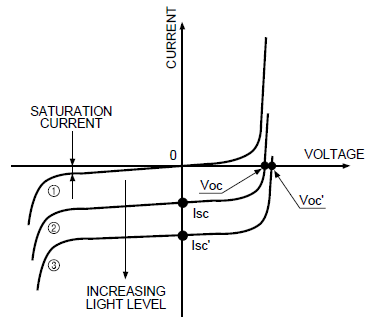
\includegraphics[scale=.6]{curve_car_phdiode}
\caption{Curve caratteristiche del fotodiodo al variare della luminosità incidente.}
\label{fig:curcar}
\end{figure}

\section{Fotodiodo VTB8440BH}

Dal datasheet del fotodiodo si possono leggere le specifiche in tabella \ref{tab:spec}.

\begin{table}[htp]
\centering
\caption{Specifiche del fotodiodo VTB8440BH}
\label{tab:spec}
\begin{tabular}{|c|c|c|}
\hline 
Grandezza & Test conditions & Valore tipico \\ 
\hline 
$I_{SC}$ & H = 100 fc, 2850 K & 5 $\mu$A \\ 
\hline 
$V_{OC}$ & 2850 K & 420 mV \\ 
\hline 
$I_D$ & H = 100 fc, 2850 K & 2 nA (max) \\ 
\hline 
$R_{SH}$ & H = 0, V = 10 mV & 70 M$\Omega$ \\ 
\hline 
$C_J$ & H = 0, V = 0 & 1 nF \\ 
\hline 
$\lambda _p$ &  & 580 nm \\ 
\hline 
NEP &  & 1.1 $\cdot$ $10^{-13}$ W/$\sqrt{Hz}$ \\ 
\hline 
D$^*$ &  & 2.2 $\cdot$ $10^{12}$ cm$\sqrt{Hz}$/W \\ 
\hline 
\end{tabular} 
\end{table}

Le prime prove sono state fatte collegando direttamente il fotodiodo al multimetro. Abbiamo dapprima impiegando il multimetro come voltmetro studiando quindi la risposta del fotodiodo in modalità fotovoltaica. Abbiamo individuato anodo e catodo del fotodiodo semplicemente guardando in che modo bisognava collegarlo per avere tensioni positive, dal momento che in caso di esposizione alla luce in modalità fotovoltaica la d.d.p. fra anodo e catodo deve essere positiva. In particolare abbiamo individuato il catodo (-) in corrispondenza di un forellino presente sul dispositivo. Abbiamo effettuato diverse misure dell'intensità luminosa in varie condizioni, in tabella \ref{tab:ill} abbiamo riportato i risultati con le relative condizioni.

\begin{table}[htp]
\centering
\caption{$V_{oc}$ (mV) in varie condizioni.}
\label{tab:ill}
\begin{tabular}{|c|c|}
\hline 
Condizione & $V_{oc}$ (mV) \\ 
\hline 
Luce lab. & 388 $\pm$ 1 \\ 
\hline 
Flash cellulare & 534 $\pm$ 5 \\ 
\hline 
Lente di ingrandimento & 400 $\pm$ 2 \\ 
\hline
Coperto con foglio di carta & 2 $\pm$ 1 \\ 
\hline  
\end{tabular} 
\end{table}

Per vedere come la risposta fotovoltaica dipenda dall'intensità luminosa abbiamo posizionato il flash della fotocamera del cellulare sul fotodiodo a varie distanze, tenendo conto che l'intensità luminosa è quadratica nella distanza (anche se non è proprio così nel caso del flash del cellulare), coprendo in parte cellulare e fotodiodo con un foglio per schermare la luce del laboratorio (misura effettivamente non essenziale). I dati sono riportati in figura \ref{fig:illum} e mostrano chiaramente come l'andamento sia non lineare. I valori ottenuti sono comunque dello stesso ordine di grandezza della $V_{oc}$ tipica riportata nel datasheet.

\begin{figure}[htp]
\centering
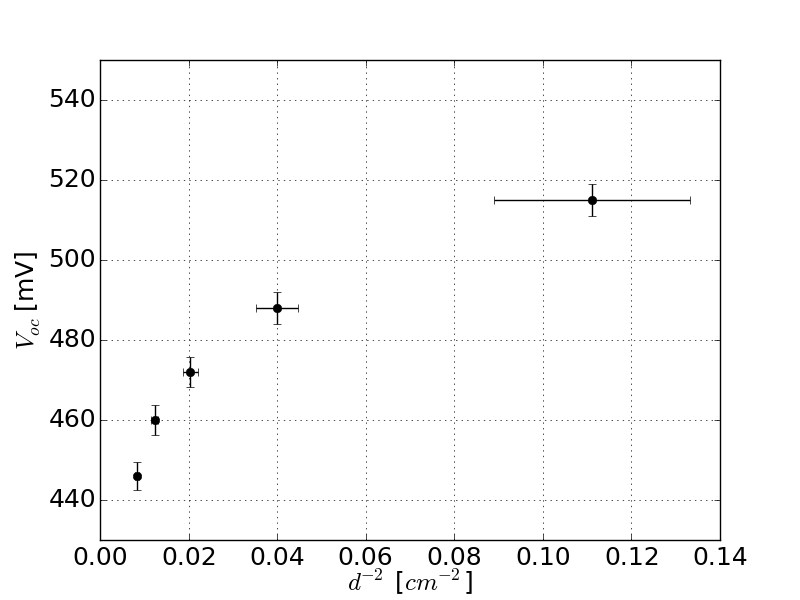
\includegraphics[scale=.4]{illum2}
\caption{Grafico di $V_{oc}$ in funzione dell'inverso della distanza al quadrato del flash.}
\label{fig:illum}
\end{figure}

Impiegando il multimetro come amperometro, in buona approssimazione i capi del fotodiodo sono cortocircuitati per cui si ha che esso lavora in modalità fotoconduttiva. In questa modalità si dovrebbe avere una dipendenza lineare dall'illuminazione, e quindi nelle ipotesi precedenti lineare con il quadrato della distanza del flash del cellulare impiegato. Abbiamo collegato l'anodo del fotodiodo all'ingresso del multimetro, per cui le crrenti osservate dovrebbero essere negative. Di fatti quello che abbiamo osservato sono state proprio correnti negative, per cui nel seguito ci si riferirà ai valori assoluti. Il valore della fotocorrente nel diodo alla luce del laboratorio, nella nostra postazione, vale I = (1.12 $\pm$ 0.01) $\mu$A, mentre il valore tipico riportato ne datasheet è 5 $\mu$A. Con le stesse modalità di prima abbiamo indagato la dipendenza della corrente dalla distanza, ottenendo il grafico in figura \ref{fig:illum_cor} in cui è evidente un andamento decisamente più lineare.

\begin{figure}[htp]
\centering
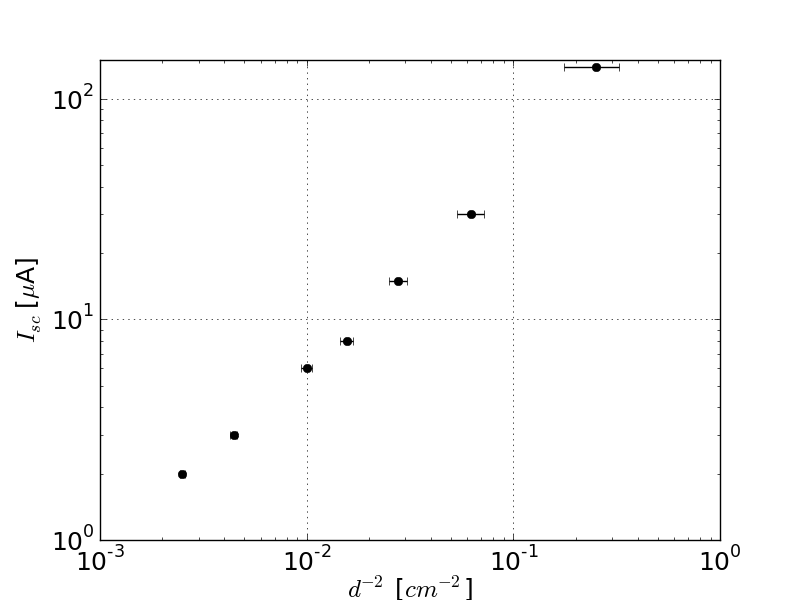
\includegraphics[scale=.4]{illum_cor2}
\caption{Grafico di $I_{sc}$ in funzione dell'inverso del quadrato della distanza.}
\label{fig:illum_cor}
\end{figure}

Dopo queste prove preliminari, abbiamo realizzato sulla breadboard il circuito in figura \ref{fig:es4}. In queste condizioni, per le regole d'oro dell'opamp il fotodiodo è in modalità fotoconduttiva poiché i suoi terminali sono alla stessa differenza di potenziale, per cui la resistenza di carico elevata consente di tradurre in tensioni che si possono agevolmente misurare delle correnti piccole come le fotocorrenti.

\begin{figure}[htp]
\centering
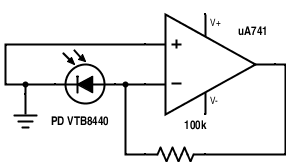
\includegraphics[scale=.6]{ES4}
\caption{Circuito realizzato per la misura delle fotocorrenti.}
\label{fig:es4}
\end{figure}

Utilizzando il VI \texttt{ACQUIS$\_$BASE$\_$2015} abbiamo misurato l'illuminazione del laboratorio. I dati sperimentali sono in figura \ref{fig:illnoncop}.

\begin{figure}[htp]
\centering
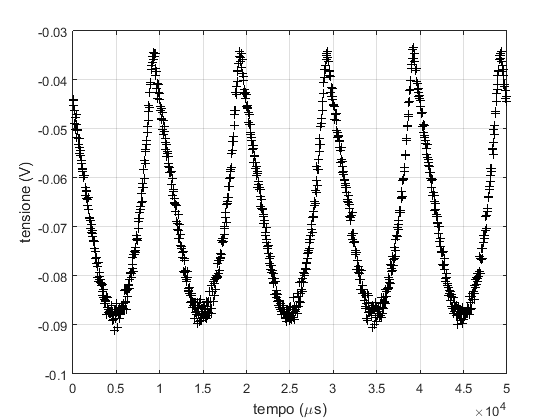
\includegraphics[scale=.5]{es4_noncoperto}
\caption{Illuminazione del laboratorio rilevata dal fotodiodo in funzione del tempo.}
\label{fig:illnoncop}
\end{figure}

Come si vede le tensioni sono negative, questo perché la fotocorrente scorre verso l'uscita dell'opamp. Il segnale osservato è periodico ad una frequenza di 100 Hz, questo perché le lampade fluorescenti del laboratorio sono alimentate da corrente alternata a 50 Hz e dal momento che l'intensità è quadratica nei campi si ottiene una frequenza principale doppia (più armoniche superiori). Il fatto che il segnale non vada a zero quando è dovuto al fatto che i tempi di reazione del gas nelle lampade sono maggiori del periodo della corrente di alimentazione, per cui non tutte le molecole del gas sono diseccitate quando la corrente è nulla. Non può essere infatti un problema di offset del fotodiodo poiché il segnale che si ottiene coprendo con dei fogli il fotodiodo varia in un intervallo compreso fra -2 mV e 6 mV, come si vede in figura \ref{fig:illumfogli}. Calcolando il valore medio e lo scarto quadratico medio si ottiene una misura dell'offset di (2217 $\pm$ 2) $\mu$V.

\begin{figure}[htp]
\centering
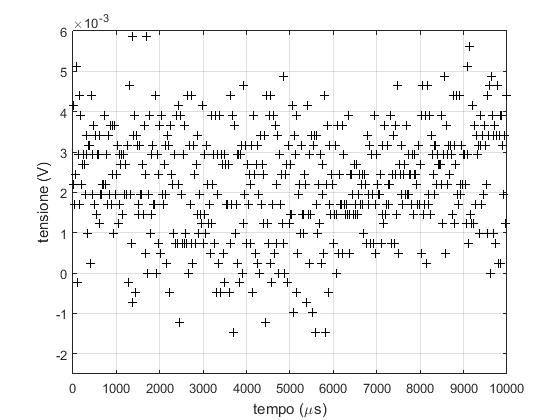
\includegraphics[scale=.5]{es4_copertofoglio_0-01_50k}
\caption{Segnale rilevato coprendo il fotodiodo con dei fogli.}
\label{fig:illumfogli}
\end{figure} 

Abbiamo infine ripetuto la misura dell'illuminazione del laboratorio con una lente di ingrandimento, facendo convergere il più possibile la luce della lampada sul fotodiodo. Come si vede in figura \ref{fig:lente}, si ottiene un segnale praticamente identico a quello di figura \ref{fig:illnoncop}, ma traslato verso il basso di circa 30 mV e con un'ampiezza di 20 mV circa maggiore, corrispondente al passaggio di più corrente nel fotodiodo e quindi ad un'illuminazione maggiore.

\begin{figure}[htp]
\centering
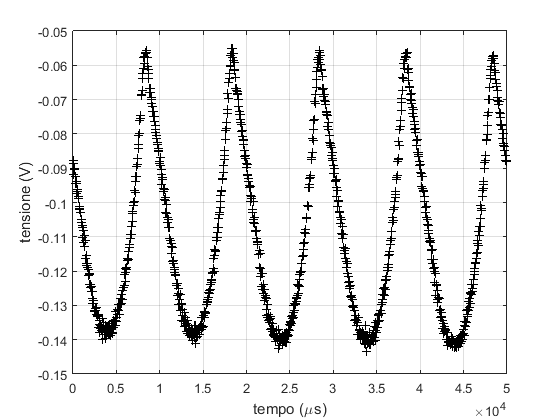
\includegraphics[scale=.5]{es4_noncoperto_lente_0-05_20k}
\caption{Illuminazione del laboratorio con lente di ingrandimento.}
\label{fig:lente}
\end{figure}

\subsection{Hm. 2}
Dal datasheet il grafico che consente la conversione fra corrente e illuminazione è quello riportato in figura \ref{fig:relcur}. Sull'asse delle coordinate viene riportata la corrente relativa, ovvero 100 volte il rapporto fra la fotocorrente misurata e il valore tipico di 5 $\mu$A riportato sul datasheet. A I$_{rel}$ = 5 $\mu$A corrisponde un'illuminazione di 100 fc.

\begin{figure}[htp]
\centering
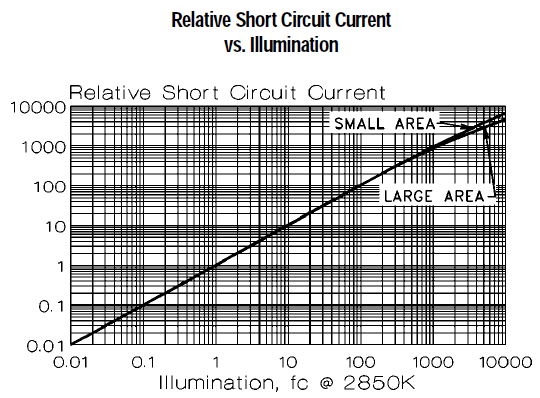
\includegraphics[scale=.5]{current}
\caption{Illuminazione vs corrente relativa.}
\label{fig:relcur}
\end{figure}

Il valor medio della corrente nel fotodiodo vale (0.674 $\pm$ 0.002) $\mu$A che dal grafico \ref{fig:relcur} corrisponde un'illuinazione di circa 13-14 fc.

\section{Fotodiodo e LED}

Poiché dal datasheet emerge che il fotodiodo ha la migliore risposta per $\lambda$ = 580 nm, abbiamo deciso di usare un LED HLPM-C315 che ha lunghezza d'onda di picco a 585 nm. Come si vede dalla figura \ref{fig:hlmp} tratta dal datasheet del LED, la luminosità cresce linearmente con la corrente a partire dai 12-13 mA, per cui nel seguito abbiamo fatto attenzione a mantenerci in questo range.

\begin{figure}[htp]
\centering
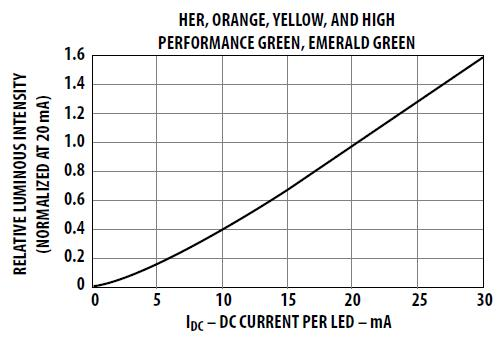
\includegraphics[scale=.6]{hlmpc315}
\caption{Intensità luminosa emessa dal LED in funzione della corrente.}
\label{fig:hlmp}
\end{figure}

Abbiamo montato sulla breadboard il circuito di alimentazione del LED. Abbiamo scelto come resistenza di carico R = 215 $\Omega$ $\pm$ 0.8 $\%$, in modo tale da poter raggiungere le correnti di lavoro. Tramite il VI \texttt{$Vin\_Vout\_2C$} abbiamo individuato il range di tensioni da applicare al LED per ottenere le correnti di interesse. Dai dati in tabella \ref{tab:curLED} si vede che per tensioni comprese fra 5 e 6 V le correnti rientrano nella regione di linearità del LED, inoltre si vede anche come la corrente dipenda linearmente dalla tensione $V_{in}$ di alimentazione.

\begin{table}
\centering
\caption{Correnti nel LED all'aumentare di $V_{in}$.}
\label{tab:curLED}
\begin{tabular}{|c|c|c|}
\hline 
$V_{in}$ (V) & $V_R$ (V)& $I_{LED}$ (mA)\\ 
\hline 
5 & 3(0) & 14 \\ 
\hline 
5.2 & 3.191(0)& 14.8 \\ 
\hline 
5.4 & 3.3812(6) & 15.7 \\ 
\hline 
5.6 & 3.569(0) & 16.6 \\ 
\hline 
5.8 & 3.7596(5) & 17.5 \\ 
\hline 
6 & 3.95(0) & 18.4 \\ 
\hline 
\end{tabular} 
\end{table}

Il LED è stato collegato ad un cavo flessibile in modo tale da poterlo posizionare direttamente sul fotodiodo. Tramite il VI \texttt{$PD\_LED$} abbiamo tracciato la caratteristica $I_{LED}~ vs~I_{PD}$, impiegando un range di tensioni da 0 V a 6 V. In figura \ref{fig:es8} sono mostrati i dati sperimentali in cui è evidente, già per basse correnti, un andamento lineare. Questo è in accordo con la risposta lineare del fotodiodo e con la dipendenza lineare dell'illuminazione emessa dal LED dalla tensione applicata, soprattutto per alte correnti.

\begin{figure}[htp]
\centering
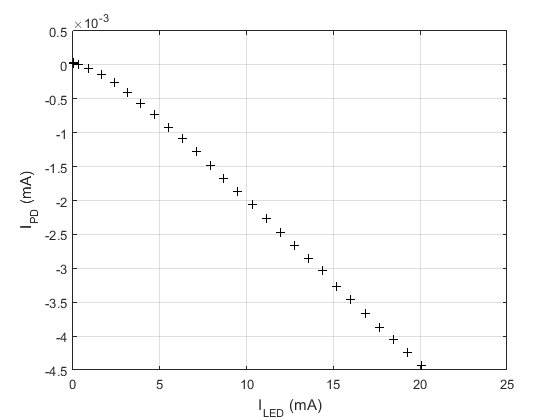
\includegraphics[scale=.5]{es8_0-6_30mis_mejo}
\caption{Caratteristica $I_{LED}~ vs~I_{PD}$ con intervallo di tensioni 0-6 V}
\label{fig:es8}
\end{figure}

\subsection{Hm. 3}
In figura \ref{fig:sens} si vede il grafico della sensitività del fotodiodo in funzione della lunghezza d'onda. Questo consente di tradurre i dati sulla corrente in termini di illuminamento del fotodiodo. Poiché il LED emette ad una lunghezza d'onda di 583 $\pm$ 15 nm, si può stimare dal grafico \ref{fig:sens} una sensitività di 0.23 $\pm$ 0.01 (A/W). 

\begin{figure}[htp]
\centering
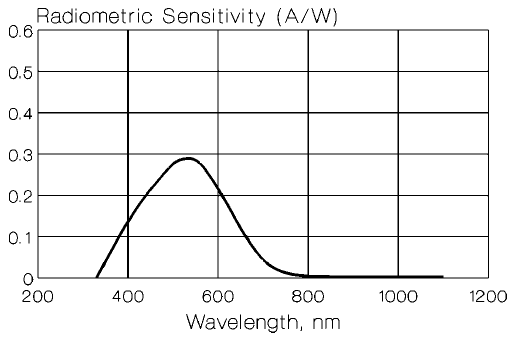
\includegraphics[scale=.5]{sensitivity}
\caption{Sensitività del fotodiodo in funzione della lunghezza d'onda.}
\label{fig:sens}
\end{figure}

Poiché 1 W vale 683 lm a 555 nm di lunghezza d'onda e dal momento che la lunghezza d'onda impiegata è simile, si può assumere valido questo fattore di conversione. Il grafico con l'illuminamento in funzione della corrente nel LED è in figura \ref{fig:illum_cor}.

\begin{figure}[htp]
\centering
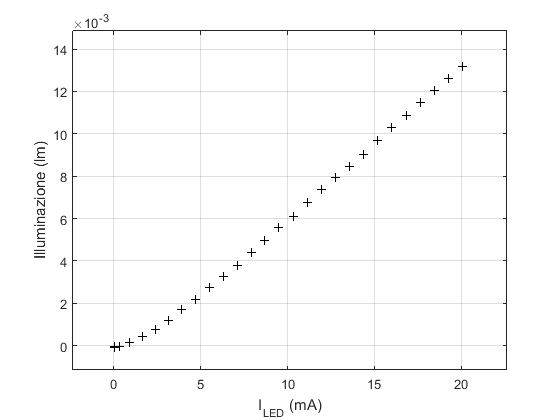
\includegraphics[scale=.5]{illum_cur}
\caption{Illuminazione sul fotodiodo in funzione della corrente nel LED.}
\label{fig:illum_cor}
\end{figure}

Abbiamo studiato la dipendenza dell'intensità luminosa al variare della distanza del LED. Per fare questo abbiamo avvolto un foglio di carta su se stesso e infilato dentro il LED, dopodiché abbiamo poggiato il rotolo sul fotodiodo e avviato il VI \texttt{$PD\_LED$} aumentando progressivamente la distanza del LED. In figura \ref{fig:dist} sono riportate le caratteristiche $I_{LED}~ vs~I_{PD}$ al variare della distanza.

\begin{figure}[htp]
\centering
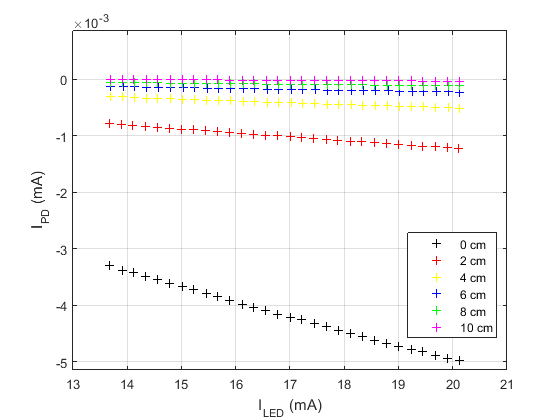
\includegraphics[scale=.6]{distance}
\caption{Caratteristica $I_{LED}~ vs~I_{PD}$ al variare della distanza del LED}
\label{fig:dist}
\end{figure}

L'ipotesi più semplice per quanto riguarda la dipendenza intensità-distanza è una legge del tipo:

\begin{equation}
\label{eqn:fit}
I = a + \frac{b}{(x-c)^2}
\end{equation}

che rende conto del fatto che il fotodiodo potrebbe avere un offset (parametro a) e che per x = 0 I resti finita (idealmente quello che si osserva ponendo il LED a contatto con il fotodiodo). Per verificare questo andamento abbiamo scelto gli ultimi dati di ciascuna curva stimando l'errore sulla corrente tramite:

\begin{equation}
\Delta I = \sqrt{(\frac{\Delta V}{R})^2 + (\frac{I\, \Delta R}{R})^2}
\end{equation}

In figura \ref{fig:discor} è riportato il fit, mentre in tabella \ref{tab:fit} i parametri fittati secondo la legge \ref{eqn:fit}.

\begin{figure}[htp]
\centering
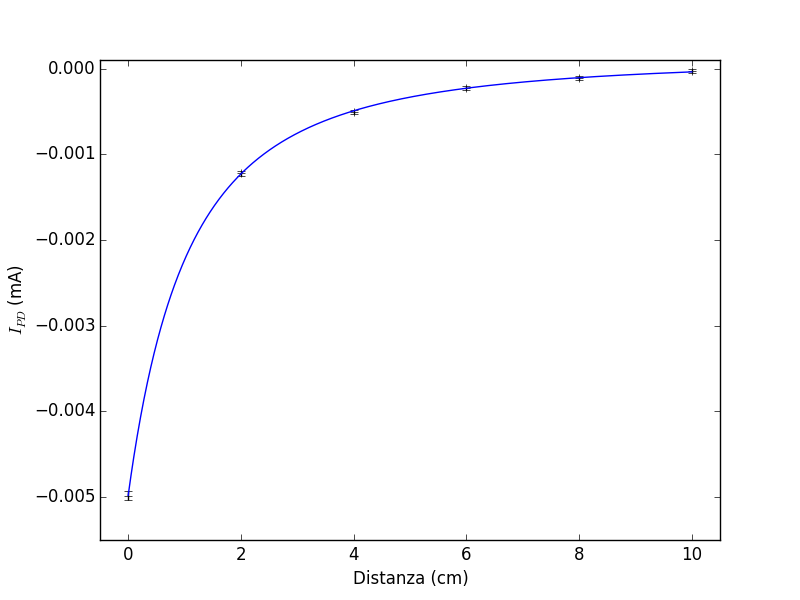
\includegraphics[scale=.4]{distanza_cor}
\caption{Fit dei dati della corrente nel fotodiodo in funzione della distanza del LED. Non sono riportati gli errori sulla distanza.}
\label{fig:discor}
\end{figure}

\begin{table}
\centering
\caption{Parametri stimati dal fit}
\label{tab:fit}
\begin{tabular}{|c|c|}
\hline 
Parametro & Valore \\ 
\hline 
a & 1.16(10) $\cdot$ $10^{-4}$ mA \\ 
\hline 
b & -0.0228(6) mA $\cdot$ cm$^2$  \\ 
\hline 
c & -2.11(3) cm \\ 
\hline 
$\chi ^2$/ndof & 0.57/3 \\ 
\hline 
\end{tabular} 
\end{table}

Si vede come l'andamento ipotizzato sia ben verificato.

\section{Fotodiodo in regime fotovoltaico}

Un fotodiodo dovrebbe obbedire all'equazione di Shockley traslata verso il basso a causa della fotocorrente:

\begin{equation}
I = I_s (\exp ^{\frac{V}{V_T}}-1)-I_{lux}
\end{equation}
 
In modalità fotovoltaica I=0 da cui:

\begin{equation}
\label{eqn:shc}
V = V_T \ln (1+\frac{I_{lux}}{I_s}) = V_T \ln (1+kI_{LED})
\end{equation} 

Dove si è sfruttata l'ipotesi verificata sperimentalmente che $I_{lux} \propto I_{LED}$. Tramite il VI \texttt{$Vin\_Vout\_2C$} abbiamo individuato la tensione di prima accensione del LED, V $\approx$ 1.36 V, e la tensione ai capi del fotodiodo oscurato, V = 0.06408 $\pm$ 0.00014 V, e alla luce del laboratorio, V = 0.3701 $\pm$ 0.0002 V.\\
Tramite il VI \texttt{$PD\_LED$} abbiamo tracciato la caratteristica $V_{OC}-I_{LED}$, dove $V_{OC}$ è la tensione al fotodiodo. In figura \ref{fig:fotov} sono mostrati i dati sperimentali: sembra evidente un andamento simile a quello previsto dall'equazione \ref{eqn:shc}.

\begin{figure}[htp]
\centering
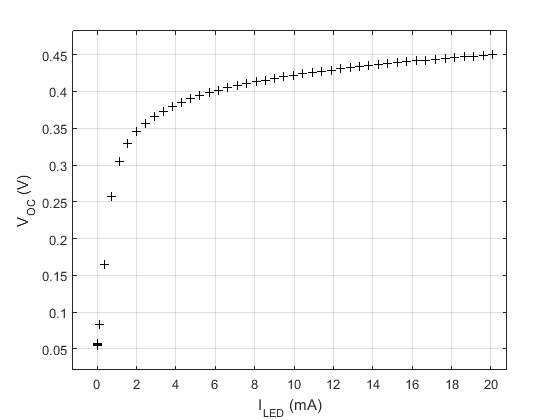
\includegraphics[scale=.6]{es12_1_6-5_50mis}
\caption{Caratteristica $V_{OC}-I_{LED}$ del fotodiodo.}
\label{fig:fotov}
\end{figure}

\subsection{Hm. 4}

Per verificare ciò abbiamo fittato i dati sperimentali tramite fit a due parametri secondo la \ref{eqn:shc}, prendendo k e $V_T$ come parametri liberi. In figura \ref{fig:hm4} è mostrato il grafico di fit, mentre in tabella \ref{tab:fithm4} i risultati del fit stesso. 

\begin{figure}[htp]
\centering
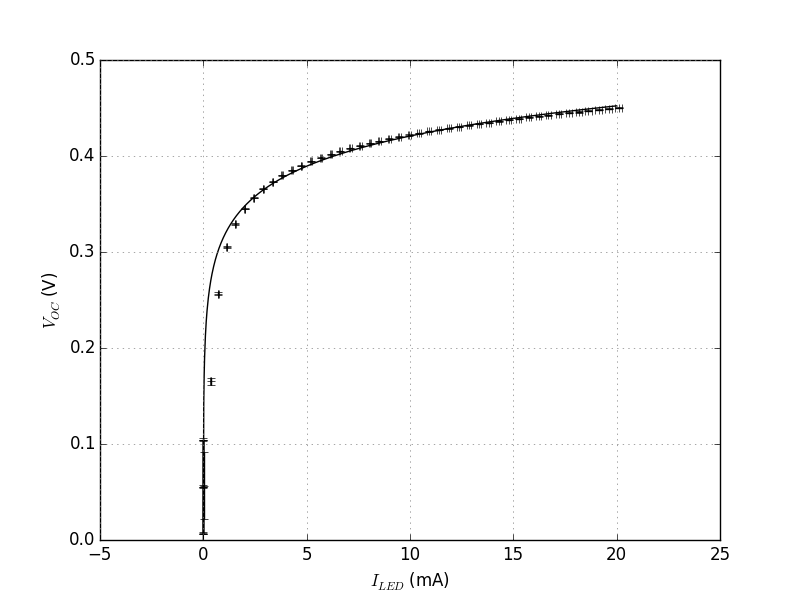
\includegraphics[scale=.4]{hm4}
\caption{Fit caratteristica $V_{OC}-I_{LED}$}
\label{fig:hm4}
\end{figure}

\begin{table}[htp]
\centering
\caption{Parametri del fit}
\label{tab:fithm4}
\begin{tabular}{|c|c|}
\hline 
Parametro & Valore \\ 
\hline 
a & 0.0453(10) V \\ 
\hline 
b & 11(2)$\cdot 10^3$ mA$^{-1}$ \\ 
\hline 
$\chi^2$/ndof & 2055/48 \\ 
\hline 
\end{tabular} 
\end{table}

Come si vede il fit segue abbastanza bene i dati sperimentali, a parte i primi dati, dove però il LED non è più in regime lineare. Se si escludono quindi le prime misure, il fit ottenuto risulta essere quello in figura \ref{fig:hm4_2} e tabella \ref{tab:fit2}. Il grafico risulta maggiormente in accordo con i dati sperimentali e il $\chi^2$ molto più ragionevole, per cui questi valori si possono considerare più significativi dei precedenti.

\begin{figure}[htp]
\centering
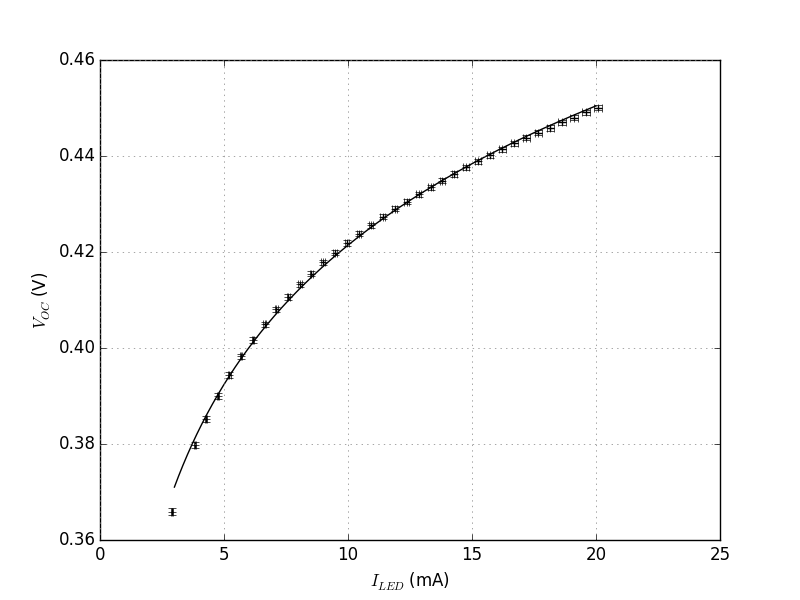
\includegraphics[scale=.4]{hm4_2}
\caption{Fit caratteristica $V_{OC}-I_{LED}$ senza le prime misure.}
\label{fig:hm4_2}
\end{figure}

\begin{table}[htp]
\centering
\caption{Parametri del fit.}
\label{tab:fit2}
\begin{tabular}{|c|c|}
\hline 
Parametro & Valore \\ 
\hline 
a & 0.0419(3) V \\ 
\hline 
b & 235(14) $\cdot 10$ mA$^{-1}$ \\ 
\hline 
$\chi^2$/ndof & 57/34 \\ 
\hline 
\end{tabular} 
\end{table}


\section{Tempi di risposta}

E' interessante valutare il tempo di risposta del fotodiodo \textsc{pdvtb8440}. Dal documento della \textit{Hamamatsu} si legge che il tempo di risposta (\textit{rise time, $t_r$}) è definito come "il tempo richiesto affinchè l'output cambi dal 10\% al 90\% del valore finale costante". In particolare, convenzionalmente si usa una sorgente luminosa a 655nm o 560nm, e una resistenza di carico di 1$k\si{Ohm}$. \\
Praticamente, è possibile, inviando al LED \textsc{hlmpc315}(la nostra sorgente di luce a 587nm) un segnale a gradino dalle opportune caratteristiche, valutare il segnale ai capi del fotodiodo: infatti, il tempo di risposta del LED (dal datasheet si legge $\tau s = 90$ns) è trascurabile rispetto a quello del fotodiodo, e nella nostra approssimazione segue fedelmente l'andamento a gradino del segnale prodotto dal generatore di funzioni. \\
Per questo motivo, ponendo il LED sulla superficie esposta del PD, questo sarà sottoposto ad un segnale luminoso a gradino, da cui ricavare il \textit{time rise}.\\
Il circuito del PD è riportato in Figura (\ref{fig:week06-es14}).

\begin{figure}
\centering
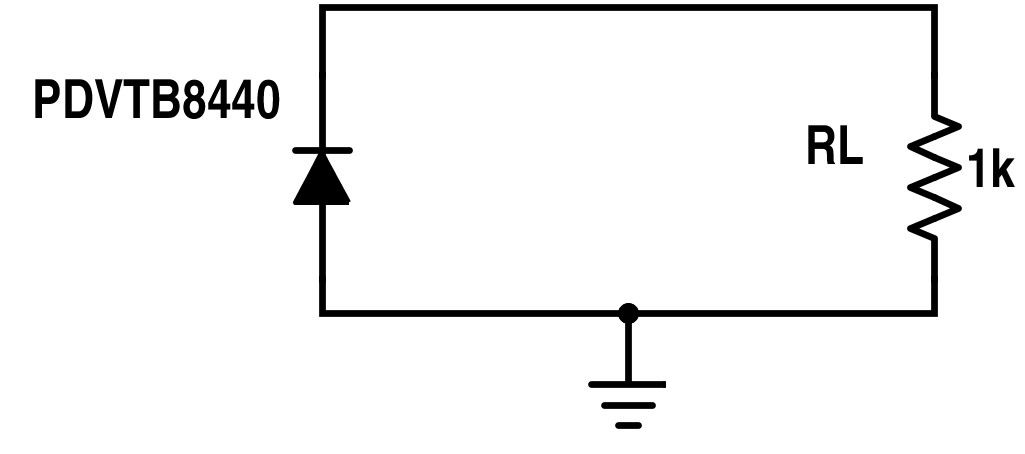
\includegraphics[width=0.9\linewidth]{./week06-es14}
\caption{Circuito di lavoro - tempi di risposta}
\label{fig:week06-es14}
\end{figure}


La prima valutazione che si può fare "a occhio" è che, a causa della capacità interna del fotodiodo da 1nF, in certi regimi di resistenze di carico si potrebbe evidenziare un comportamento affine a quello del tempo di risposta di un filtro RC, dove il $\tau $ è proporzionale al prodotto $R_L C$, con $R_L$ resistenza di carico.\\
Studiando il grafico \textbf{Rise/fall Times - Non Standard} riportato nel \textit{datasheet} del fotodiodo \textsc{vtb8440}, sembra che l'andamento del rise time, nella regione circa compresa fra 10-100 $R_L C [\mu s]$ corrisponda ad una relazione funzionale circa lineare, con pendenza unitaria, per cui uguale a quella di un filtro RC. Nessuna informazione è invece data per valori $R_L C [\mu s]$ maggiori di 100.\\

Viene chiesto di esplorare un range di resistenze fra $10 \si{k Ohm} - 5.6 \si{M Ohm}$: notiamo subito che, fissata la capacità C=1nF, questo corrisponde a all'intervallo nella scala delle ascisse del grafico in esame di $(1-5600 [\mu s])$, ben al di là del limite riportato. Per questo motivo, abbiamo deciso di scegliere resistenze ben equispaziate nel range 1-100 $R_L C [\mu s]$, e alcune maggiori di tale valore.\\

I punti sperimentali da noi trovati sono riportati nei grafici (\ref{fig:rise_time_1-100}, \ref{fig:rise_time_all}, \ref{fig:rise_time_all_logx}) con varie scale.\\

\begin{figure}
\centering
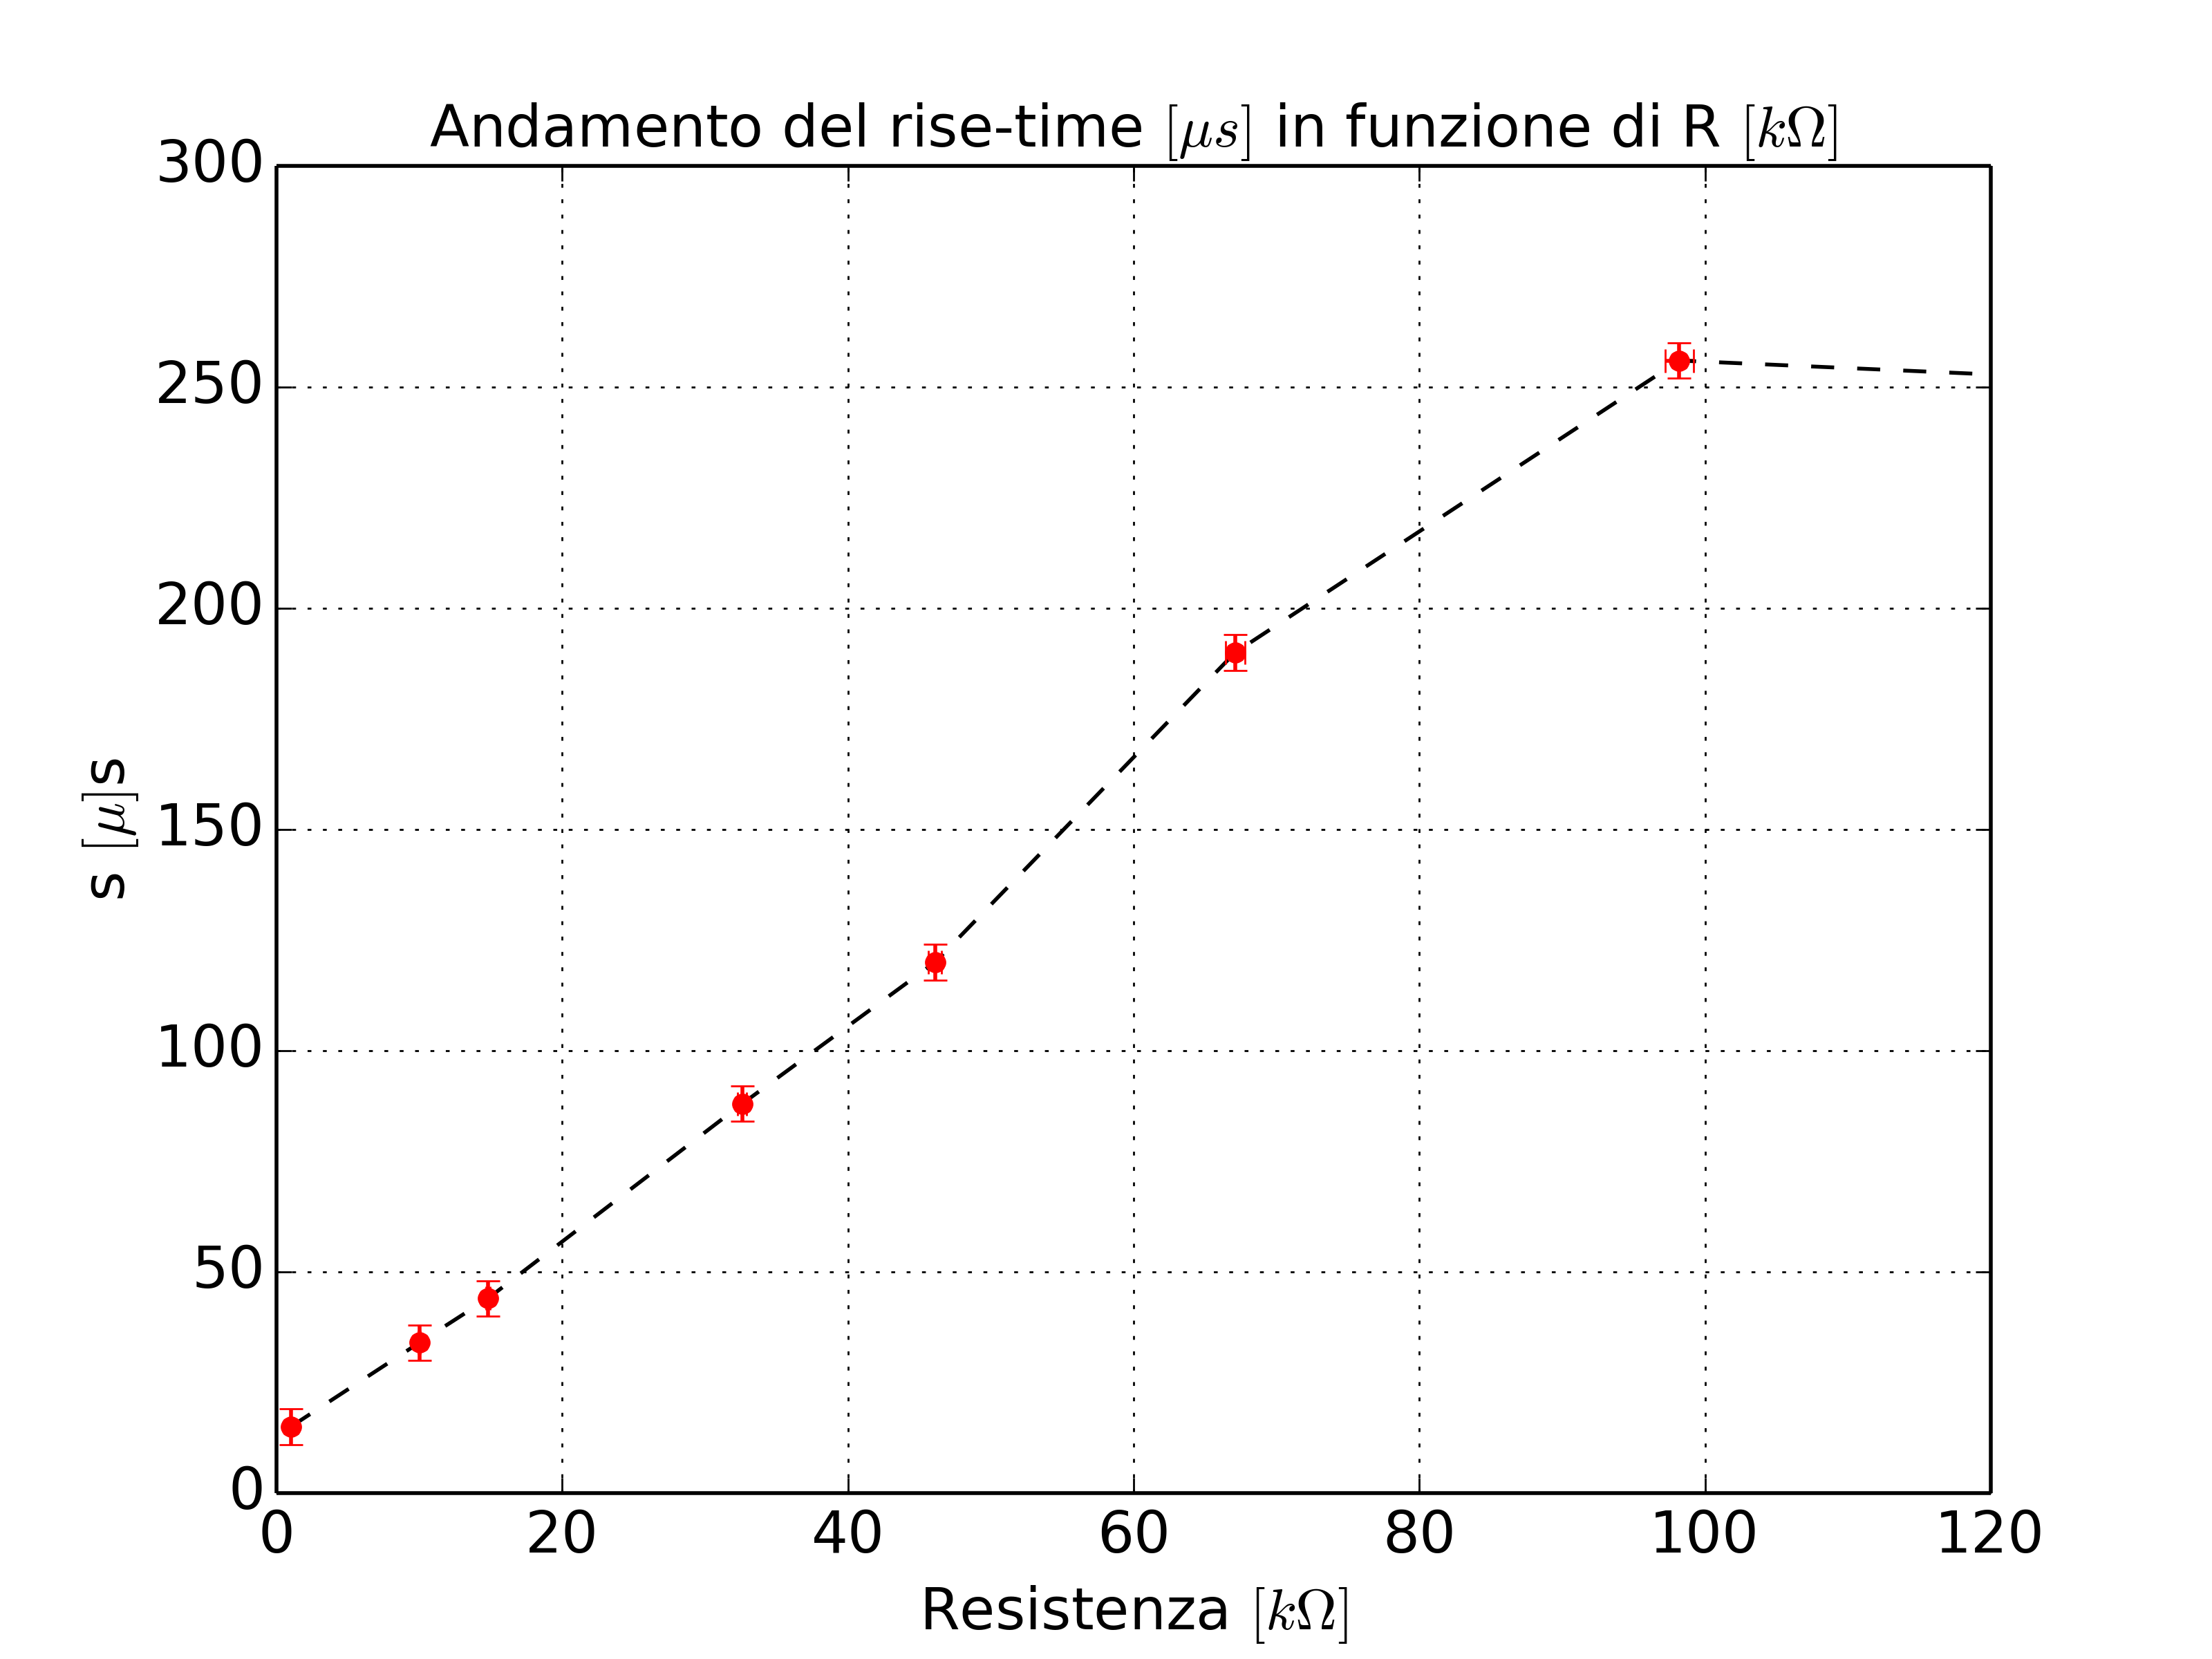
\includegraphics[width=0.8\linewidth]{./rise_time_1-100}
\caption{Rise-time in funzione della resistenza $R_L$ (valori RC fra 1-100)}
\label{fig:rise_time_1-100}
\end{figure}

\begin{figure}
\centering
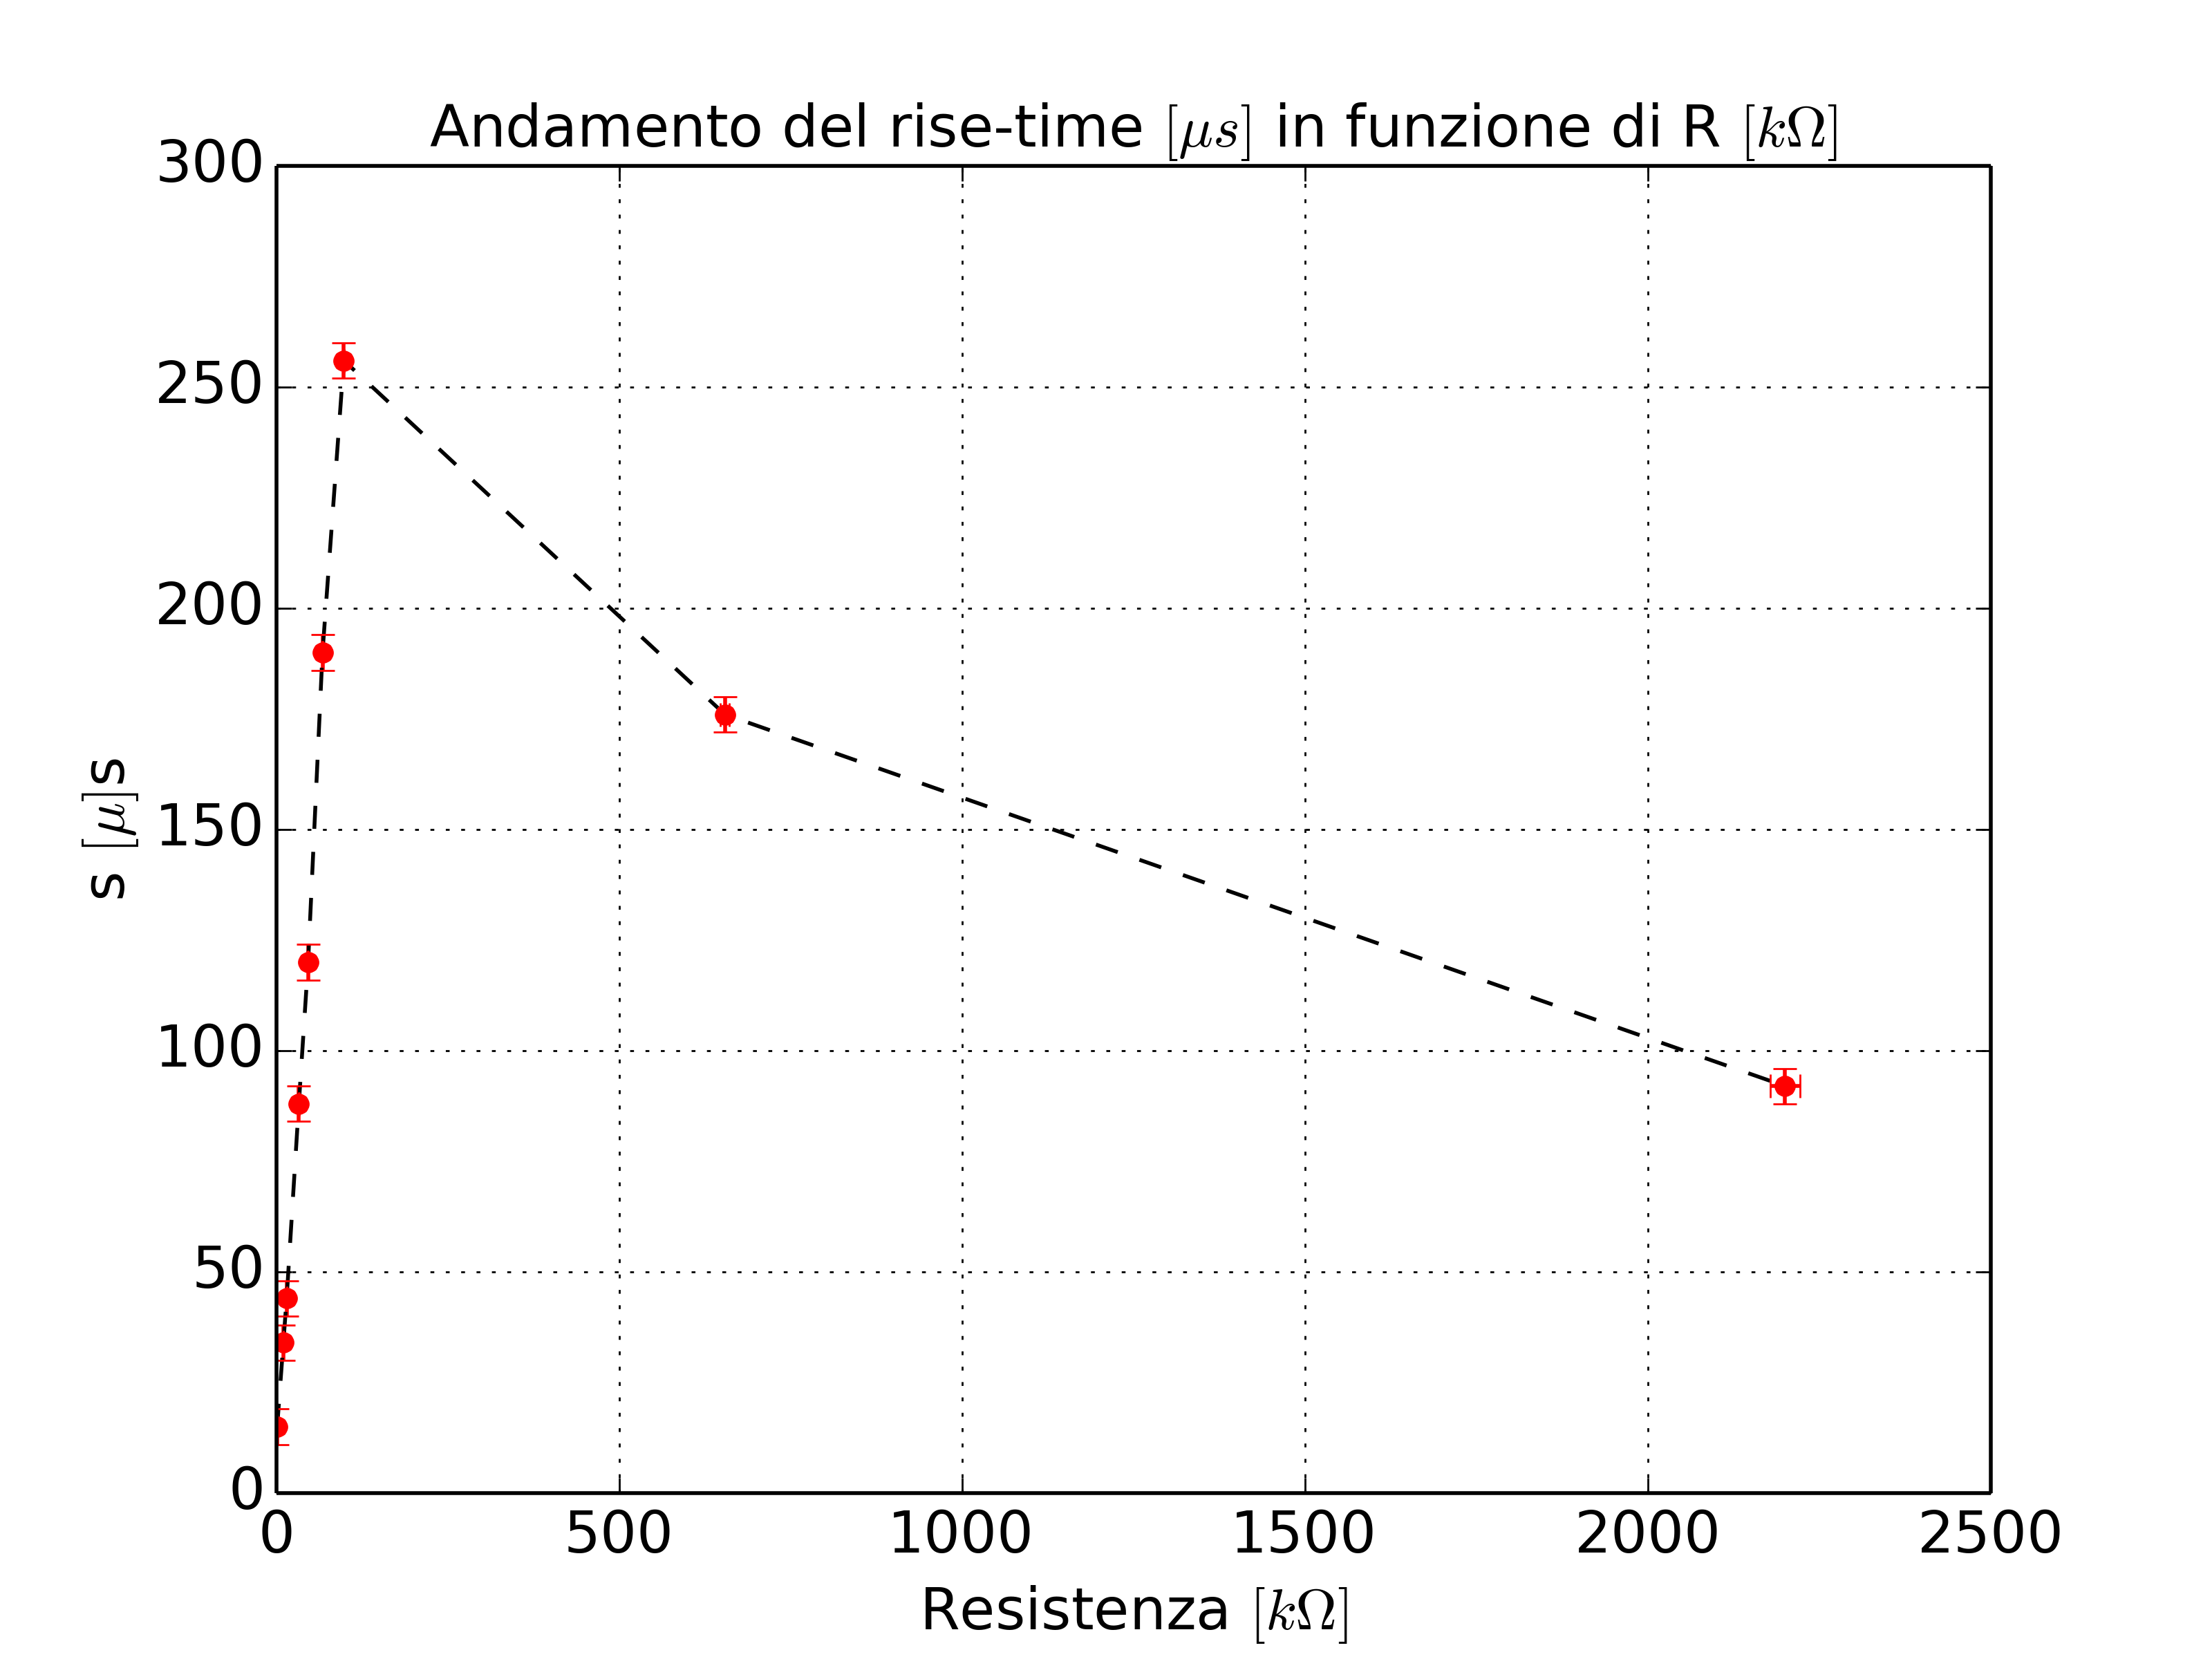
\includegraphics[width=0.8\linewidth]{./rise_time_all}
\caption{Rise-time in funzione della resistenza - serie completa di dati, scala lineare}
\label{fig:rise_time_all}
\end{figure}

\begin{figure}
\centering
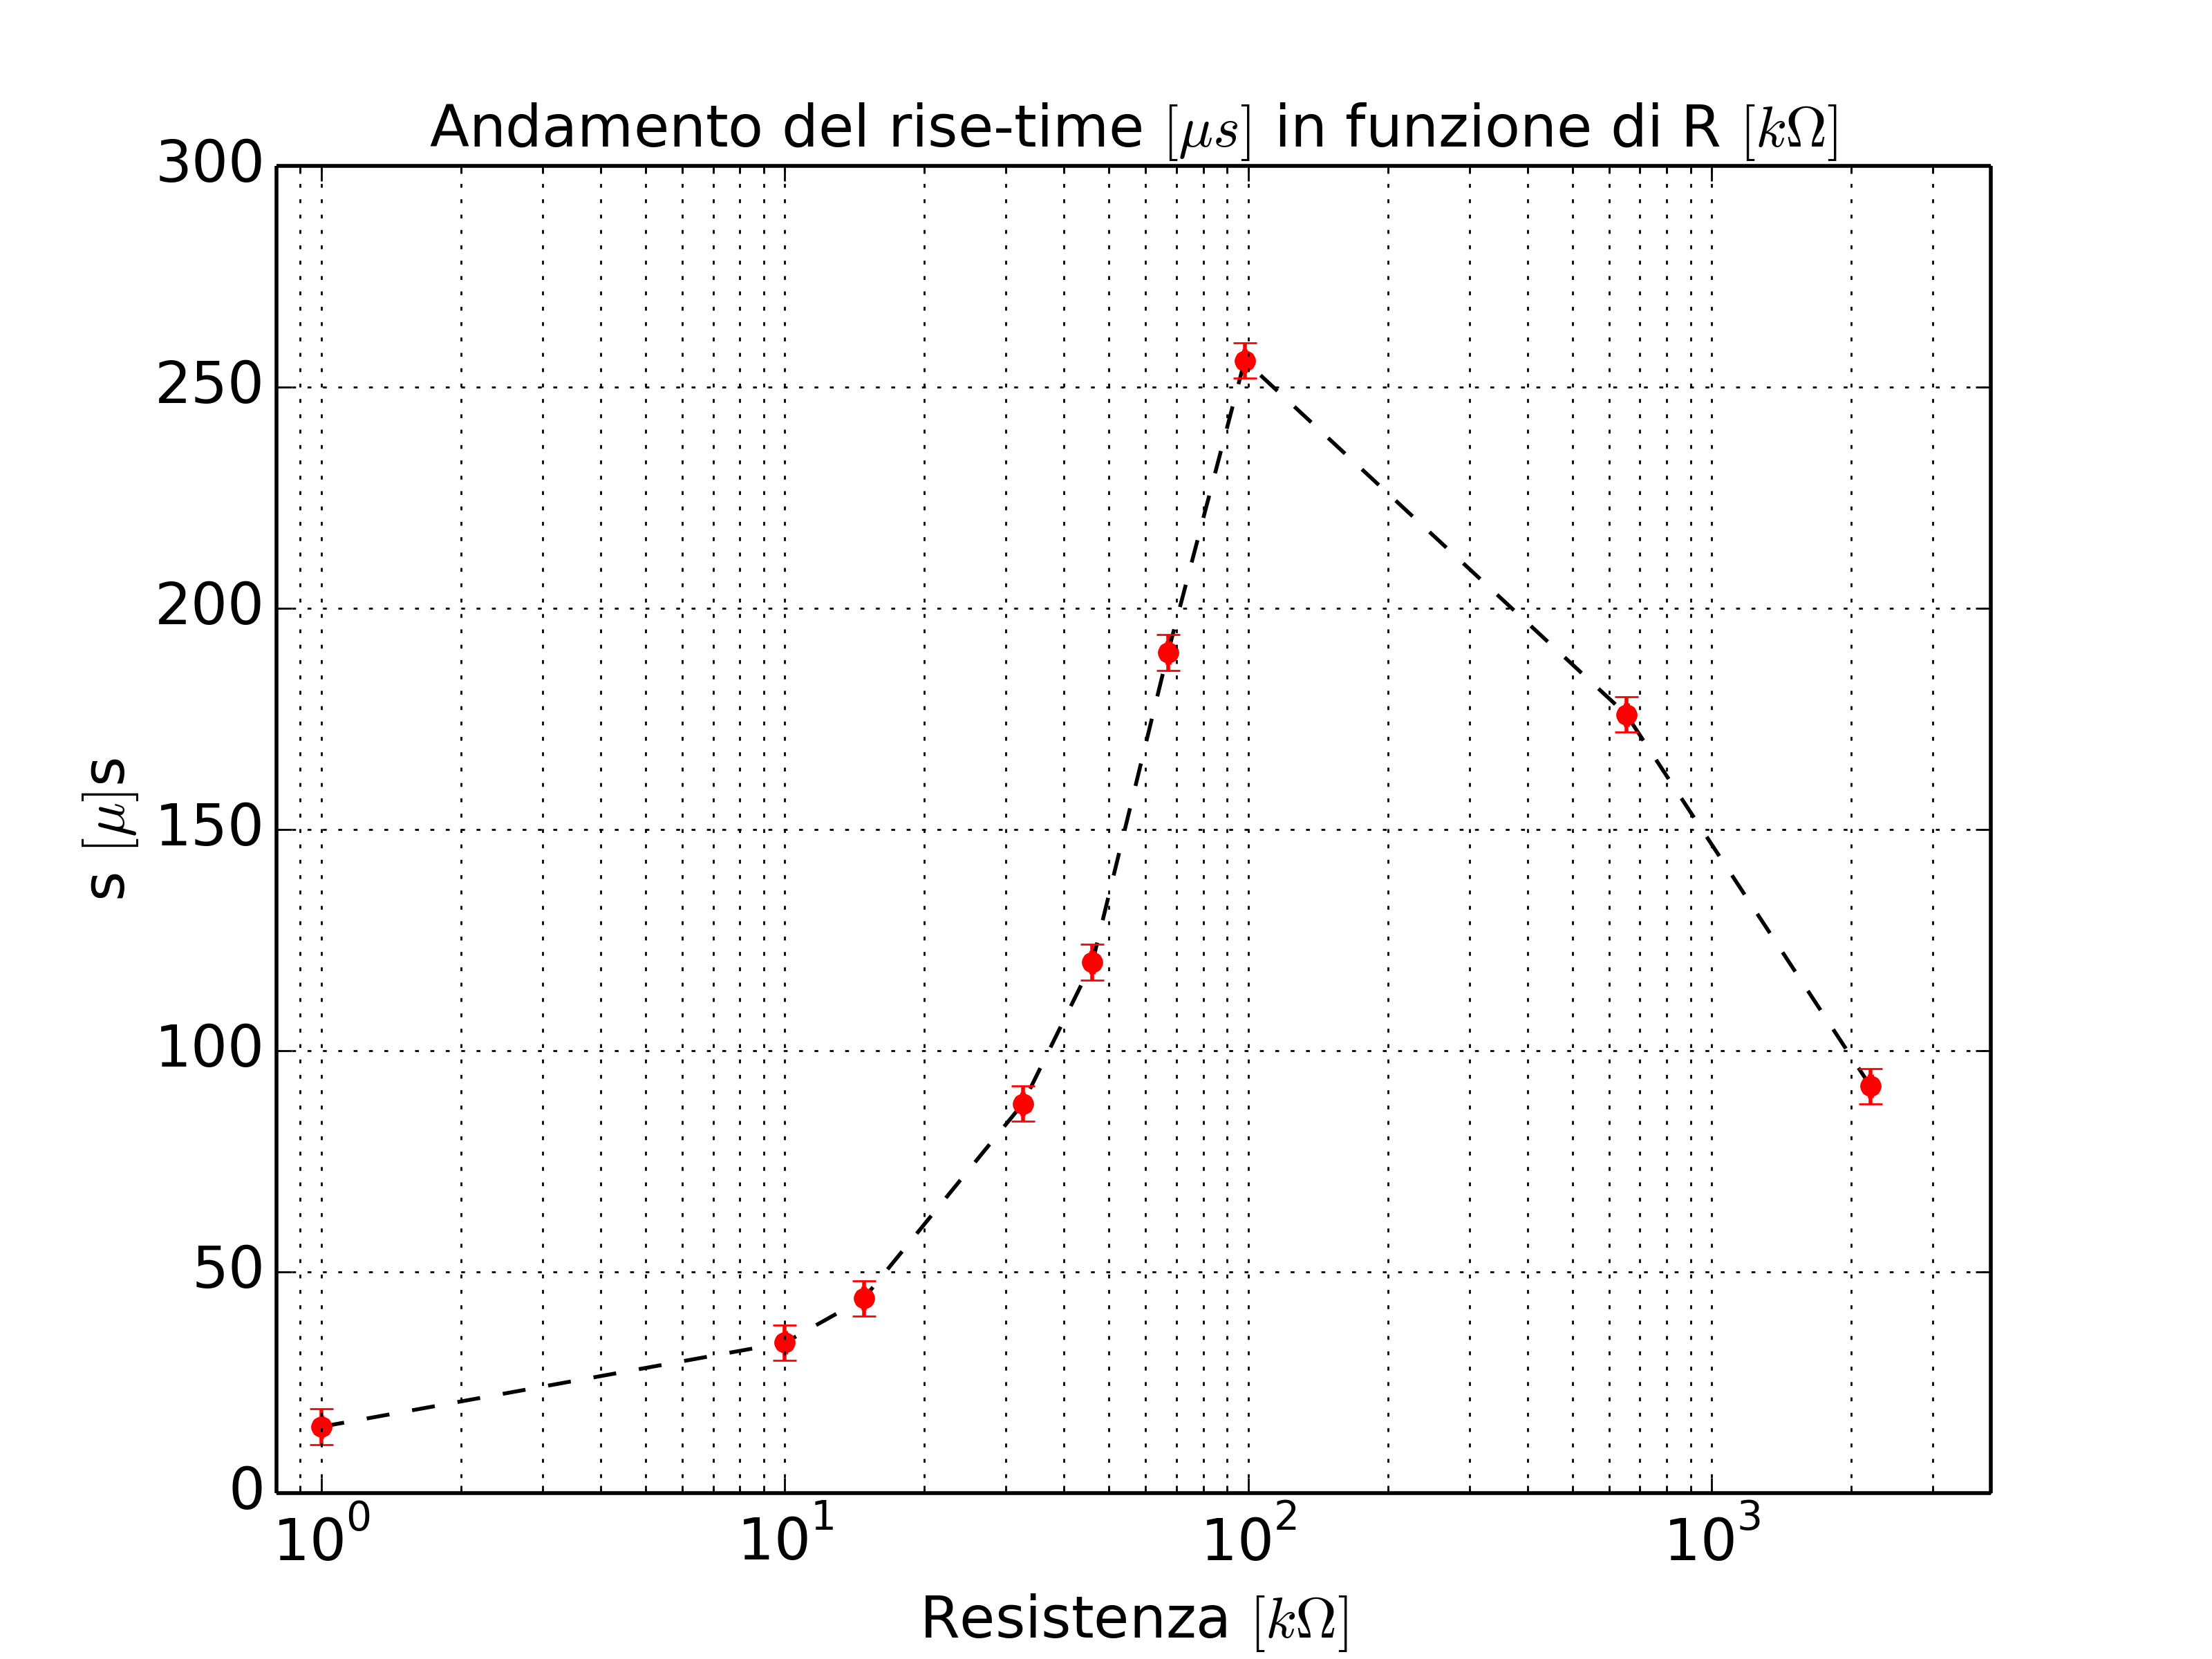
\includegraphics[width=0.8\linewidth]{./rise_time_all_logx}
\caption{Rise-time in funzione della resistenza - serie completa di dati, scala logx}
\label{fig:rise_time_all_logx}
\end{figure}


Si verifica che nell'intervallo indicato nel datasheet, effettivamente l'andamento previsto è ben rispettato, al contrario, si vede come aumentando il carico oltre 100k$\Omega$ il rise time diminuisca sensibilmente, in aperto contrasto con il modello di filtro RC introdotto prima.\\

Annotiamo alcune considerazioni importanti:

\begin{itemize}
\item Dalle forme del segnale acquisito dal VI \textsc{acquis\_base\_2015}, si nota un progressivo scostamento fra la fase di salita e quella di discesa, con quest'ultima che presenta una forte somiglianza con il processo di scarica di un condensatore al punto che, per alte resistenze, e prima della successiva fase di risalita, sembra permanere una carica residua sulle armature. 

\item Per valutare accuratamente i tempi di risalita, così come indicato nel documento \textit{Hamamatsu}, in primo luogo si è effettuata una stima visiva, esaminando il grafico prodotto dal VI, e successivamente si è proceduto ad interpolare con Octave i dati sperimentali, impiegando la funzione \textbf{interp1}, e scegliendo come metodo di interpolazione l'impiego di un polinomio definito "a pezzi" (\textit{piece-wise polynomial}) composto ciascuno da polinomi dispari di Hermite di quarto grado, tali da preservare la forma dei dati. Il risultato è notevole ed è riportato un esempio in Figura (\ref{fig:es14_10vpp_33k_hermite}), con i dati acquisiti usando un carico da 32.6 k$\Omega$.
\end{itemize}

\begin{figure}
\centering
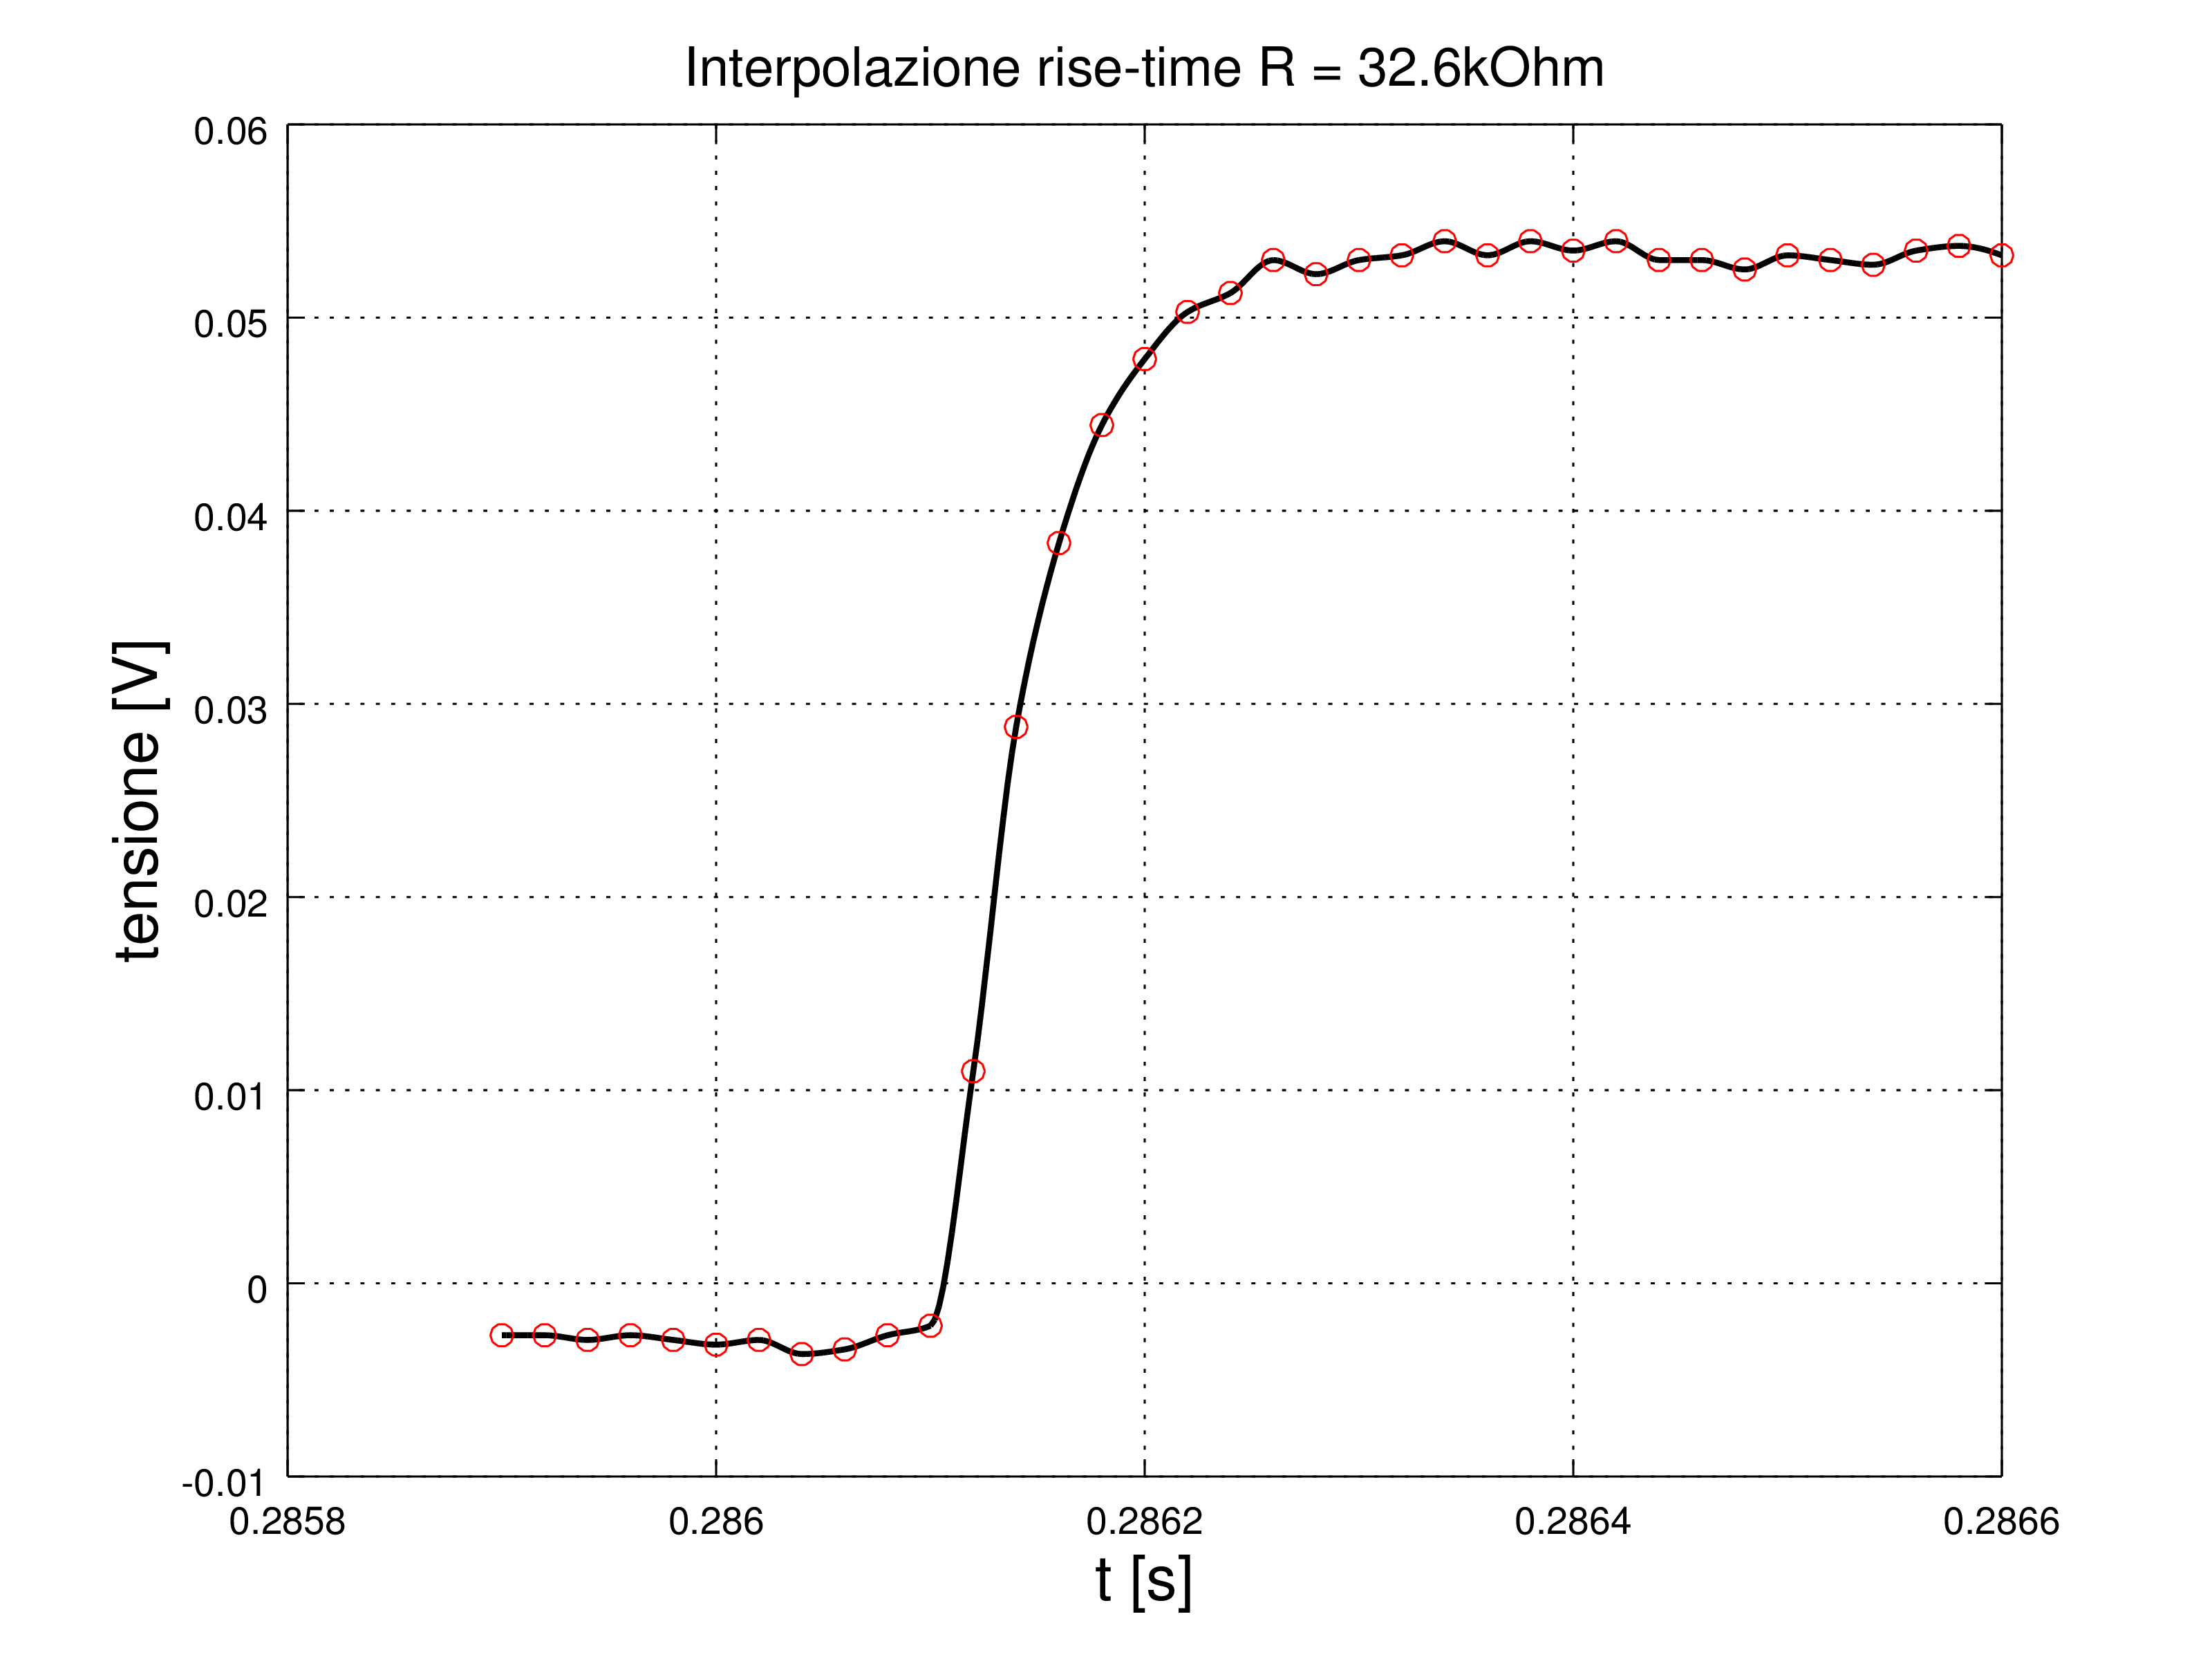
\includegraphics[width=0.8\linewidth]{./es14_10vpp_33k_hermite}
\caption{Interpolazione del rise time con Hermite piecewise polynomials}
\label{fig:es14_10vpp_33k_hermite}
\end{figure}


\section{Risposta ad un impulso in regime fotoconduttivo}

Ricolleghiamo nuovamente il fotodiodo al circuito amplificante, composto dall'op-amp precedentemente impiegato e la transresistenza di 100k$\Omega$; il circuito è presentato in Figura (\ref{fig:es15-week06-a}). Si vuole valutare qual è la risposta ad un impulso a circuito chiuso, quindi in regime fotoconduttivo. Il risultato, in Figura (\ref{fig:rispo_impulso_multiplot}-a), è simile a quanto riportato sul documento \textit{Hamamatsu} in Figure 4-2(b).

\begin{figure}
\centering
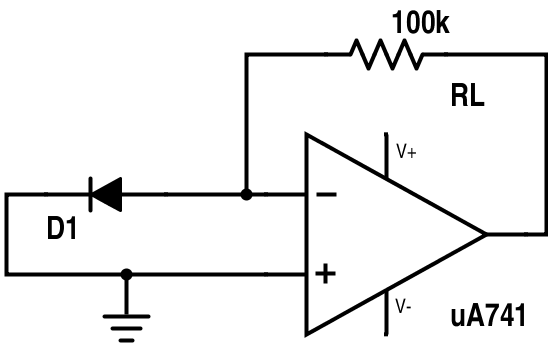
\includegraphics[width=0.8\linewidth]{./es15-week06-a}
\caption{Circuito con amplificatore a transresistenza - configurazione A}
\label{fig:es15-week06-a}
\end{figure}

\begin{figure}
\centering
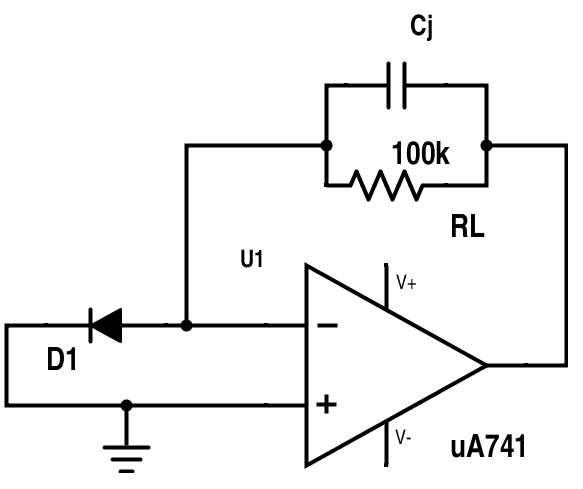
\includegraphics[width=0.8\linewidth]{./es15-week06-b}
\caption{Circuito con amplificatore a transresistenza - configurazione B}
\label{fig:es15-week06-b}
\end{figure}



L'aver collegato i due ingressi dell'op-amp ai terminali del fotodiodo fa si che, quando illuminato, quest'ultimo crei una differenza di potenziale tra \textsc{in+} e \textsc{in-}, che dovrà essere compensata dall'operazionale in modo da annullarla. A far questo ci pensa ovviamente il circuito di feedback che però, a causa della capacità interna al fotodiodo, introduce delle oscillazioni ad alta frequenza, visibili nell'output. Questo fenomeno è detto di \textit{gain ringing}.\\
Provando, come suggerito, a collegare in parallelo alla transresistenza una capacità $C_j$ (vedi Figura (\ref{fig:es15-week06-b})le oscillazioni ad alte frequenze dovrebbero essere smorzate molto più in fretta. In Figura (\ref{fig:rispo_impulso_multiplot}) è riportato un multiplot con gli output ottenuti per vari valori di $C_j$: il segnale da noi visualizzato, purtroppo, è risultato troppo rumoroso (a causa delle basse tensioni in uso) per poter osservare chiaramente il comportamento atteso, tuttavia si "intuisce" (per alcune configurazioni più chiaramente che per altre) uno smorzamento progressivamente maggiore delle oscillazioni ad alte frequenze all'aumentare della capacità $C_j$.

\begin{figure}
\centering
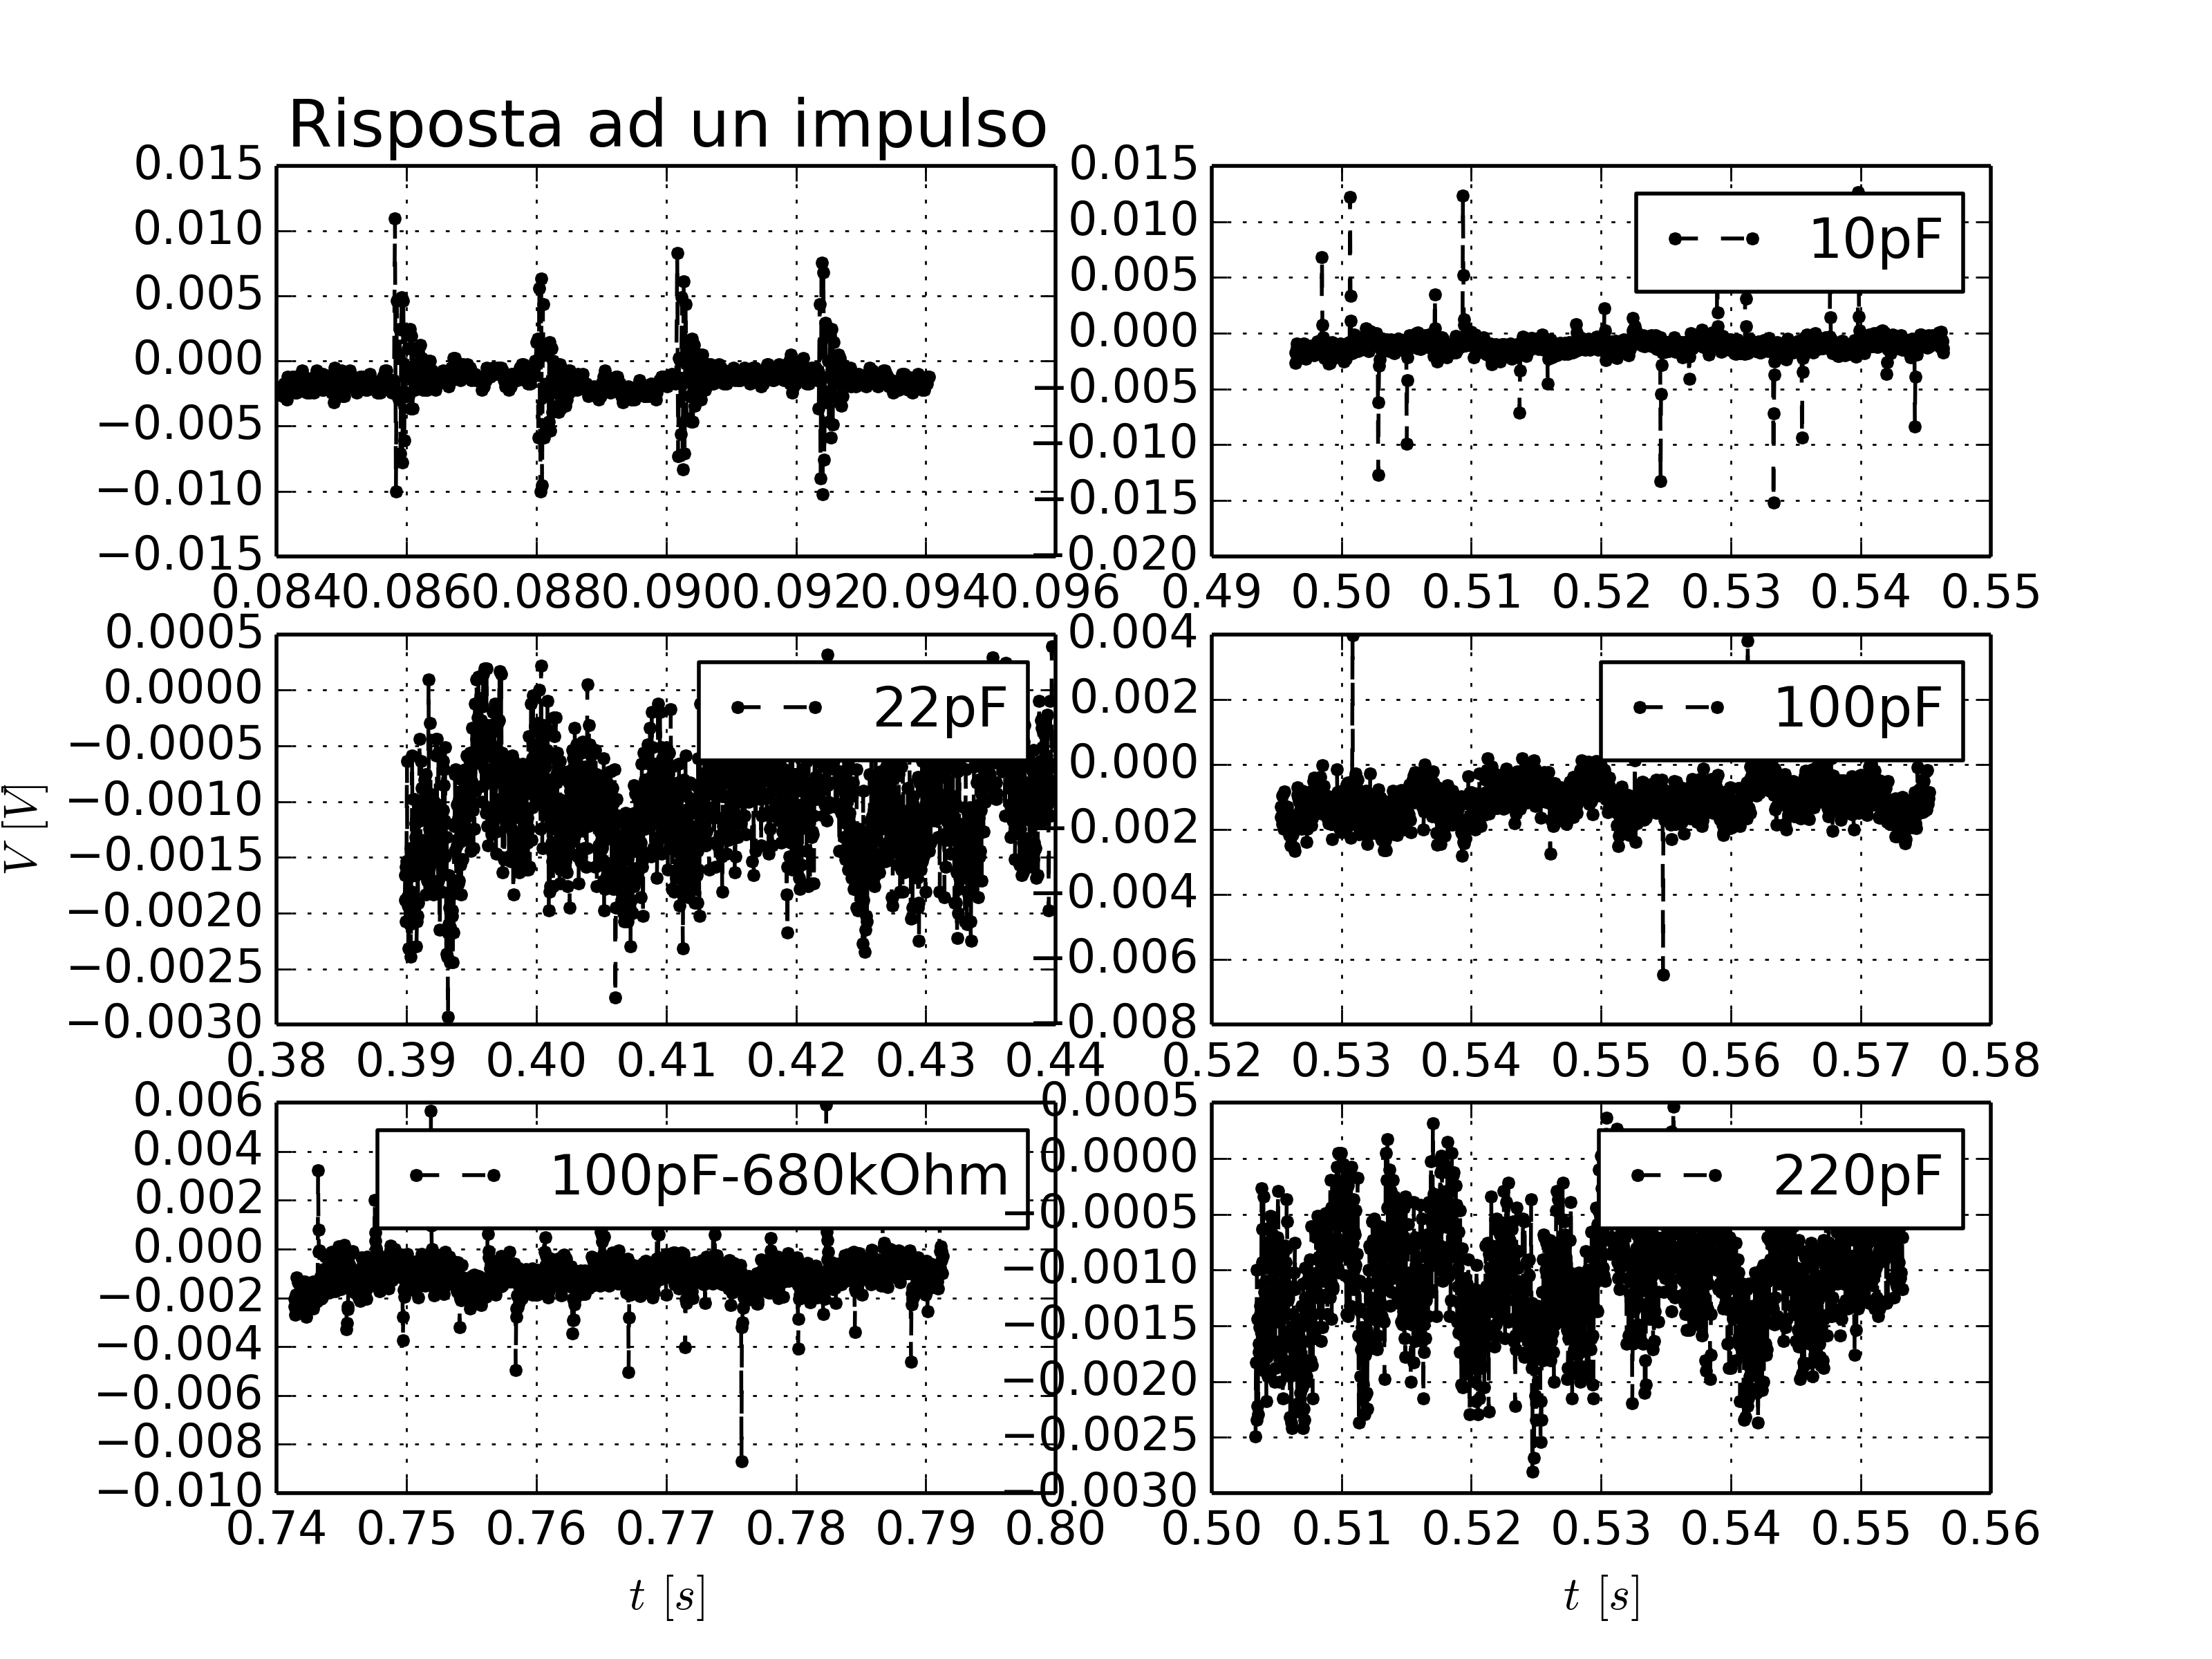
\includegraphics[width=0.9\linewidth]{./rispo_impulso_multiplot}
\caption{Multi-plot circuito a transresistenza in risposta ad un segnale impulsivo, con il fenomeno dei gain-ringing ben visibile}
\label{fig:rispo_impulso_multiplot}
\end{figure}



\section{Fotocellula VT935G}

In poche parole, una fotocellula è un dispositivo a semiconduttore capace di variare la sua resistenza interna in base all'intensità del segnale luminoso che riceve sulla giunzione esposta. In particolare, la resistenza è massima a condizione di luminosità nulla e diminuisce progressivamente all'aumentare di questa. La fotocellula a nostra disposizione è prodotta dalla Perkin-Elmer, di modello \textsc{vt935g}. Sono riportati di seguito i parametri ritenuti più importanti tratti dal datasheet:\\

\begin{tabular}{|c|c|c|}
\hline \textbf{Parameter} & \textbf{Rating} & \textbf{Units} \\ 
\hline Cont. Pow. Dissipation & 80 & mW \\ 
\hline Temp. range & da -40 a +75 & C \\ 
\hline Resistance @10lux & 18.5-40.5 & k$\Omega$ \\ 
\hline Resistance (dark) min & 1 & M$\Omega$ \\ 
\hline Max. voltage & 100 & V \\ 
\hline Response Time (@1fc) & 35(rise)/5(fall) & ms \\ 
\hline 
\end{tabular} 

~\\
Usando il tester in modalità ohmetro, valutiamo dei valori di resistenza in varie condizioni di luminosità:\\

\begin{tabular}{|c|c|}
\hline \textbf{Luminosità} & \textbf{Resistenza} \\ 
\hline luce ambiente  & 4.5 $\pm 0.2 \si{kOhm}$ \\ 
\hline foglio di carta & 1.8 $\si{MOhm}$ \\ 
\hline dentro astuccio & $ \geq 80 \si{MOhm}$ \\ 
\hline 
\end{tabular} 

~\\

Possiamo utilizzare questi dati per valutare anche in questo caso l'illuminazione della stanza, sfruttando il parametro $\gamma$ definito come la pendenza della retta che passa per due punti arbitrari del grafico \textit{Resistance vs Illumination}, in scala bilog. La ditta Perkin-Elmer prende come punti convenzionali 10 lux (0.93fc) e 100 lux (93fc), a cui corrispondono le resistenze $R_{10}$ e $R_{100}$. S veda Figura (\ref{fig:logres_vs_logill}). Dal datasheet della fotocellula \textsc{vt935g} si ricava $\gamma = 0.9$, e $R_{10} = 18.5/29/40 k\Omega$ (in base alle tre diverse tipologie della fotocellula in uso).\\

\begin{figure}
\centering
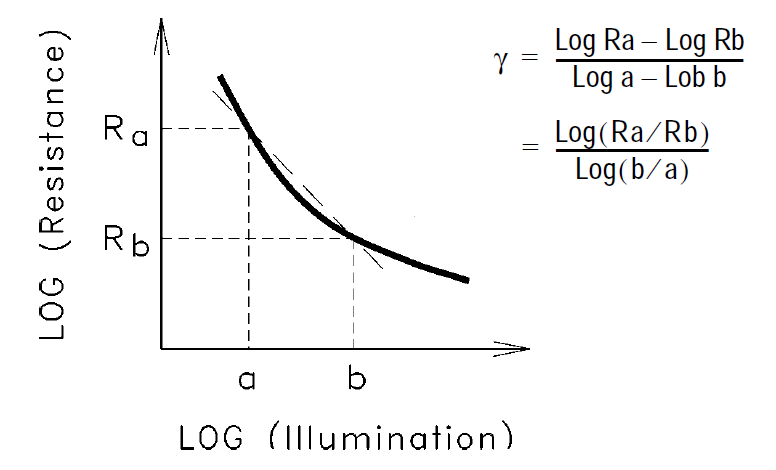
\includegraphics[width=0.9\linewidth]{./logres_vs_logill}
\caption{Definizione del parametro $\gamma$ e grafico logRes-loglum}
\label{fig:logres_vs_logill}
\end{figure}

Sfruttando queste relazioni, e approssimando la curva con la retta per la regione di luminosità compresa fra 10-100 lux, possiamo scrivere:

\begin{equation}
x[lux] = 10[lux](\frac{R_{10}}{R_x})^{0.9}
\end{equation}

dove ovviamente vale l'analogo per le luminosità espresse in fc.
Dato che, in linea di principio, non sappiamo distinguere quale fra il gruppo A, B, C è quello di appartenenza della fotocellula, abbiamo tre diversi valori di illuminazione $x$, con l'errore su $R_x$ propagato correttamente:\\

\begin{tabular}{|c|c|c|}
\hline \textbf{Group} & \textbf{Illumination(lux)} & \textbf{Illumination (fc)} \\ 
\hline A & 48(2) & 4.47(19) \\ 
\hline B & 79(4) & 7.37(37) \\ 
\hline C & 113(5) & 10.54(47) \\ 
\hline 
\end{tabular} 
 
~\\


\subsection{Hw. 6}
Al pari dei fotodiodi, le fotocellule sono dei disposotivi a semiconduttore capaci di rilevare la luminosità ambientale. Tuttavia, questi si distinguono a livello costruttivo poichè i fotodiodi sono basati su una o più \textit{giunzioni}, mentre le fotocellule si basano sul \textit{bulk effect} e in particolare sul fatto che la resistività del \textit{bulk} diminuisca all'aumentare dell'illuminazione. \\
Una conseguenza importante di questo differente funzionamento, è ben visibile se consideriamo la Figura (\ref{fig:hw6_compare_pd_pr}), dove sono confrontati le caratteristiche I-V di entrambi i dispositivi.\\ 
Una delle caratteristiche principali delle fotocellule è, quindi, quella di avere un comportamento lineare fra corrente e tensione, simmetrico per valori negativi e per circuiti in DC o in AC. Altri punti di forza sono il basso costo, la buona responsività ad alte e basse illuminazioni, l'amplissima gamma di valori di resistenze in commercio, il basso rumore, la responsività a quasi tutte le lunghezze d'onda del visibile.\\


\begin{figure}
\centering
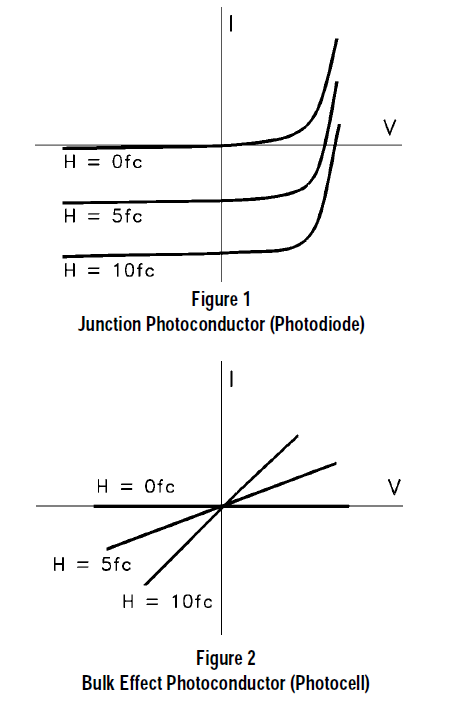
\includegraphics[width=0.7\linewidth]{./hw6_compare_pd_pr}
\caption{Confronto fra le caratteristiche I-V di un fotodiodo (in alto) e una fotocellula (in basso)}
\label{fig:hw6_compare_pd_pr}
\end{figure}

Le applicazioni sono quindi numerose e variano dal controllo dell'esposizione delle macchine fotografiche, a quello della densità del toner nelle fotocopiatrici; possono essere usate per controllare l'illuminaazione stradale e anche dei sensori di posizione. \\
Uno dei circuiti più semplici in cui possono essere impiegate le fotocellule è ad esempio un sensore di luminosità ambientale che sfrutta un amplificatore della tensione prodotta ai capi della fotoresistenza (vedi Figura (\ref{fig:hw6_sens_lum})).Un ulteriore uso delle fotocelle è nei circuiti di AC/DC relay, o nei sensori di movimento.

\begin{figure}
\centering
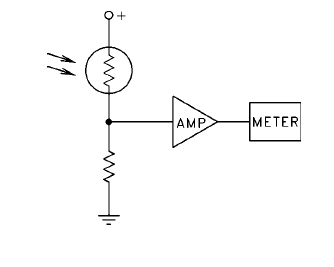
\includegraphics[width=0.8\linewidth]{./hw6_sens_lum}
\caption{Sensore di luminosità ambientale.}
\label{fig:hw6_sens_lum}
\end{figure}


Possiamo utilizzare la fotocellula a nostra disposizione per costruire un circuito con un LED che si accenda/spenga in base alle condizioni di illuminazione della fotocellula. Ad esempio, montando un circuito come in Figura (\ref{fig:es-18-week06}) si fa in modo che, all'aumentare dell'intensità luminosa, la fotoresitenza sia sempre più piccola fino a quando la corrente che passa per il LED non è tale da permettere una sua accensione. Con un circuito leggermente diverso, invece (mostrato in Figura (\ref{fig:week06-es20})), si può ottenere un comportamento opposto, cioè in cui al diminuire della luminosità ambientale venga attivato il LED. Ovviamente è necessario fornire una tensione di alimentazione prossima a quel valore di "soglia" in modo che una piccola variazione produca degli effetti visibili.

\begin{figure}
\centering
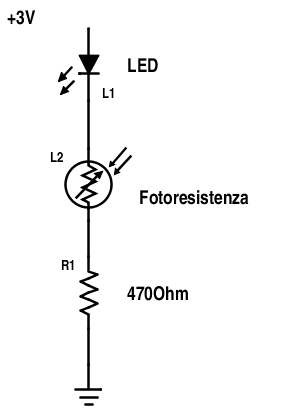
\includegraphics[width=0.5\linewidth]{./es-18-week06}
\caption{Circuito usato per valutare la resistenza della fotoresistenza}
\label{fig:es-18-week06}
\end{figure}


\begin{figure}
\centering
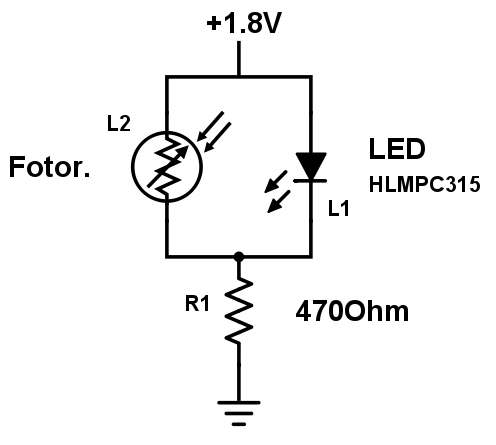
\includegraphics[width=0.7\linewidth]{./week06-es20}
\caption{Circuito: al diminuire della luminosità ambientale il LED si accende.}
\label{fig:week06-es20}
\end{figure}


\section{Caratteristica resistenza-illuminazione}

E' interessante valutare con maggiore precisione la resistenza della fotocellula in funzione dell'illuminazione, fornita sempre dal LED. Per far questo, è stato proposto un circuito come quello in Figura (\ref{fig:es23-week06}), dove nel ramo della fotoresistenza vi è un partitore di tensione con resistenza di carico $R$ fissa in modo che, detta $FR$ la fotoresistenza, si possa scrivere:

\begin{equation}\label{fr}
FR = R \frac{V_{in}-V_{out}}{V_{out}}
\end{equation}

dove $V_{out}$ è la tensione letta ai capi del carico $R$.

\begin{figure}
\centering
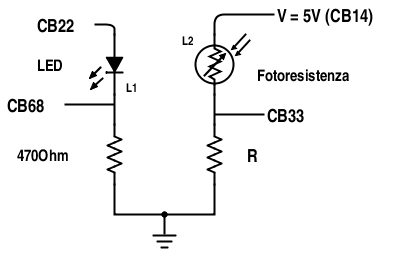
\includegraphics[width=0.8\linewidth]{./es23-week06}
\caption{Circuito per la visualizzazione della caratteristica resistenza-illuminazione}
\label{fig:es23-week06}
\end{figure}


Per dimensionare adeguatamente la resistenza di carico in modo da ottenere una misura quanto più precisa possibile di $FR$ si possono fare dei semplici ragionamenti:

\begin{itemize}
\item Se $R$ fosse troppo più piccola, $V_{out}$ sarebbe vicina al valore di terra, quindi molto più piccola di $V_{in}$, rendendola difficile da misurare e soprattutto amplificherebbe notevolmente l'incertezza sul valore di $FR$ finale.

\item Se, al contrario, $R$ fosse troppo più grande di $FR$, si potrebbe potenzialmente verificare un fenomeno di cancellazione al numeratore del membro a destra della (\ref{fr}), poichè ciò implicherebbe che $V_{out} \simeq V_{in}$. Anche in questo caso, il calcolo di $FR$ potrebbe essere afflitto da grande incertezza.


\end{itemize}

Scegliendo invece un carico dello stesso ordine di grandezza, la fotoresistenza verrebbe valutata in modo ottimale. Infatti, viene suggerito in seguito di usare una resistenza da 10k$\si{Ohm}$ come carico del circuito, verificando che la corrente e la potenza dissipata nella fotocellula siano entro i limiti indicati nel datasheet.\\
Il calcolo di queste due quantità è stato effettuato per una resistenza di carico un poco inferiore a $10 \si{kOhm}$ (da 5.58 $\si{kOhm}$) e risulta $I \simeq 0.5$mA, $P \simeq 2.5$mW, ampiamente al di sotto dei valori massimi riportati nel datasheet.

Fissato un fondoscala da 5V, l'errore da attribuire a $FR$ sarebbe, dunque:

\begin{equation}
(\Delta FR)^2 = (\frac{\Delta V_{in} + \Delta V_{out}}{V_{in} - V_{out}})^2 + (\frac{\Delta V_{out}}{V_{out}})^2 + (\frac{\Delta R}{R})^2 \simeq (FR/100)^2
\end{equation}

Cercando nel documento \textbf{PhotocellIntroduction.pdf}, il grafico a cui fare riferimento, per poterlo confrontare con i dati che andremo ad acquisire della resistenza $FR$ in funzione della corrente che scorre nel LED, si trova a pag.9 e viene riportato di seguito in Figura (\ref{fig:res_versus_illumi}). Per una certa regione compresa fra 0.1-10 fc le curve mostrano un coefficiente angolare circa pari a 1, per cui ci aspettiamo una relazione fra $FR$ e \textit{Illumination} che va circa come $FR \sim [Ill]^{-1}$.\\

\begin{figure}
\centering
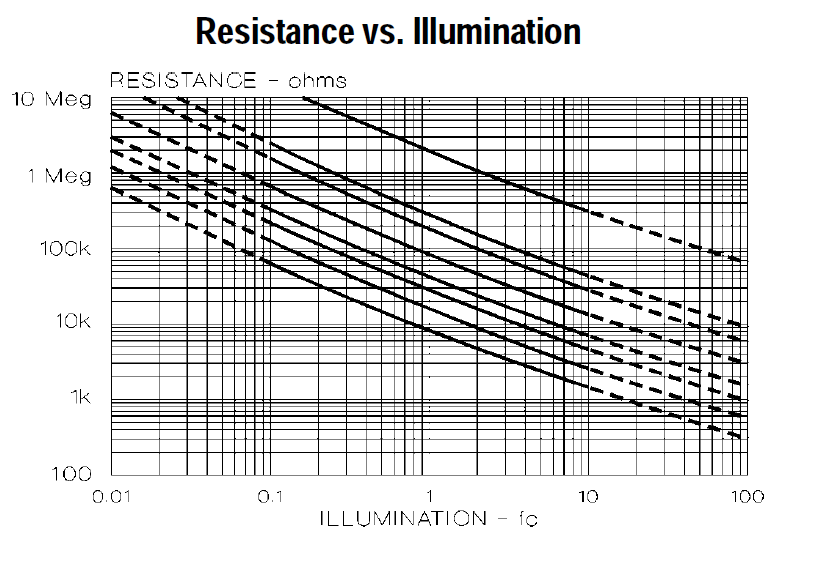
\includegraphics[width=0.9\linewidth]{./res_versus_illumi}
\caption{Andamento della resistenza della fotocellula in funzione della illuminazione - scala bilog}
\label{fig:res_versus_illumi}
\end{figure}

Nel nostro caso, però, sulle ascisse abbiamo la corrente che circola nel LED, quindi riprendiamo un risultato osservato nella parte precedente dell'esperienza e cioè la diretta proporzionalità fra l'illuminazione e la \textit{short circuit current}, che ci permette di legare in maniera facile i due grafici (in Figura (\ref{fig:short_current_vs_illum}) è riportato il grafico \textbf{Relative Short Circuit Current vs. Illumination} tratto dal datasheet \textit{fotodiodoVTB8440}).\\

\begin{figure}
\centering
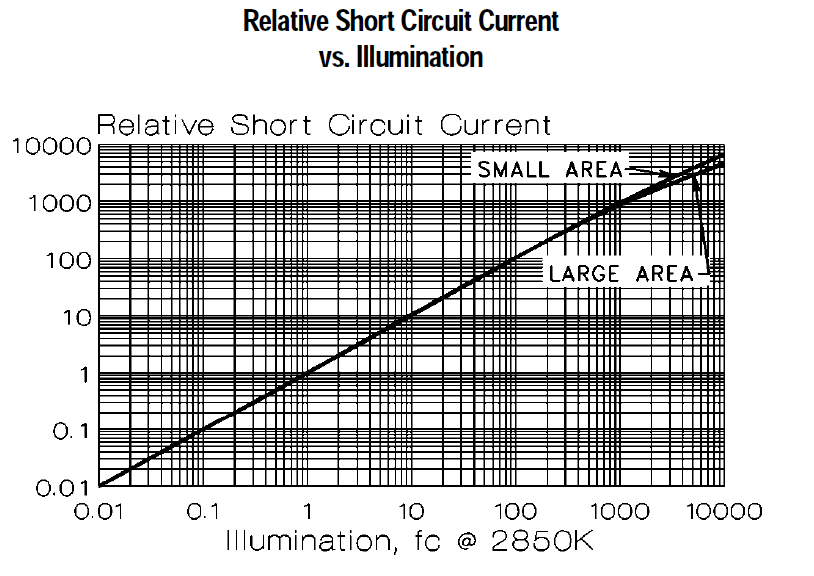
\includegraphics[width=0.9\linewidth]{./short_current_vs_illum}
\caption{Corrente a circuito chiuso in funzione dell'illuminazione del fotodiodo VTB8440 - le scale sono relative e in bilog.}
\label{fig:short_current_vs_illum}
\end{figure}

Ora possiamo riportare, quindi, i risultati della nostra acquisizione con resistenza di carico $R = 10\si{k Ohm}$: il valore della fotoresistenza quando la corrente nel LED satura a $I_{LED} = 14.6 mA$ è di $FR = 2.03 \pm 0.02 k\si{Ohm}$. Cosa più importante, l'andamento dei dati ricalca molto bene quello previsto, sia in scala lineare che loglog (si vedano i grafici riportati in Figura (\ref{fig:plot_FR_vs_ill}), (\ref{fig:plot_FR_vs_ill_loglog})). Purtroppo, a causa del fatto che il grafico (\ref{fig:short_current_vs_illum}) è in unità arbitrarie, non si riescono a trarre delle informazioni utili relative all'effettiva illuminazione sulla fotocellula capace di produrre una resistenza dell'ordine dei 2k$\Omega$.

\begin{figure}
\centering
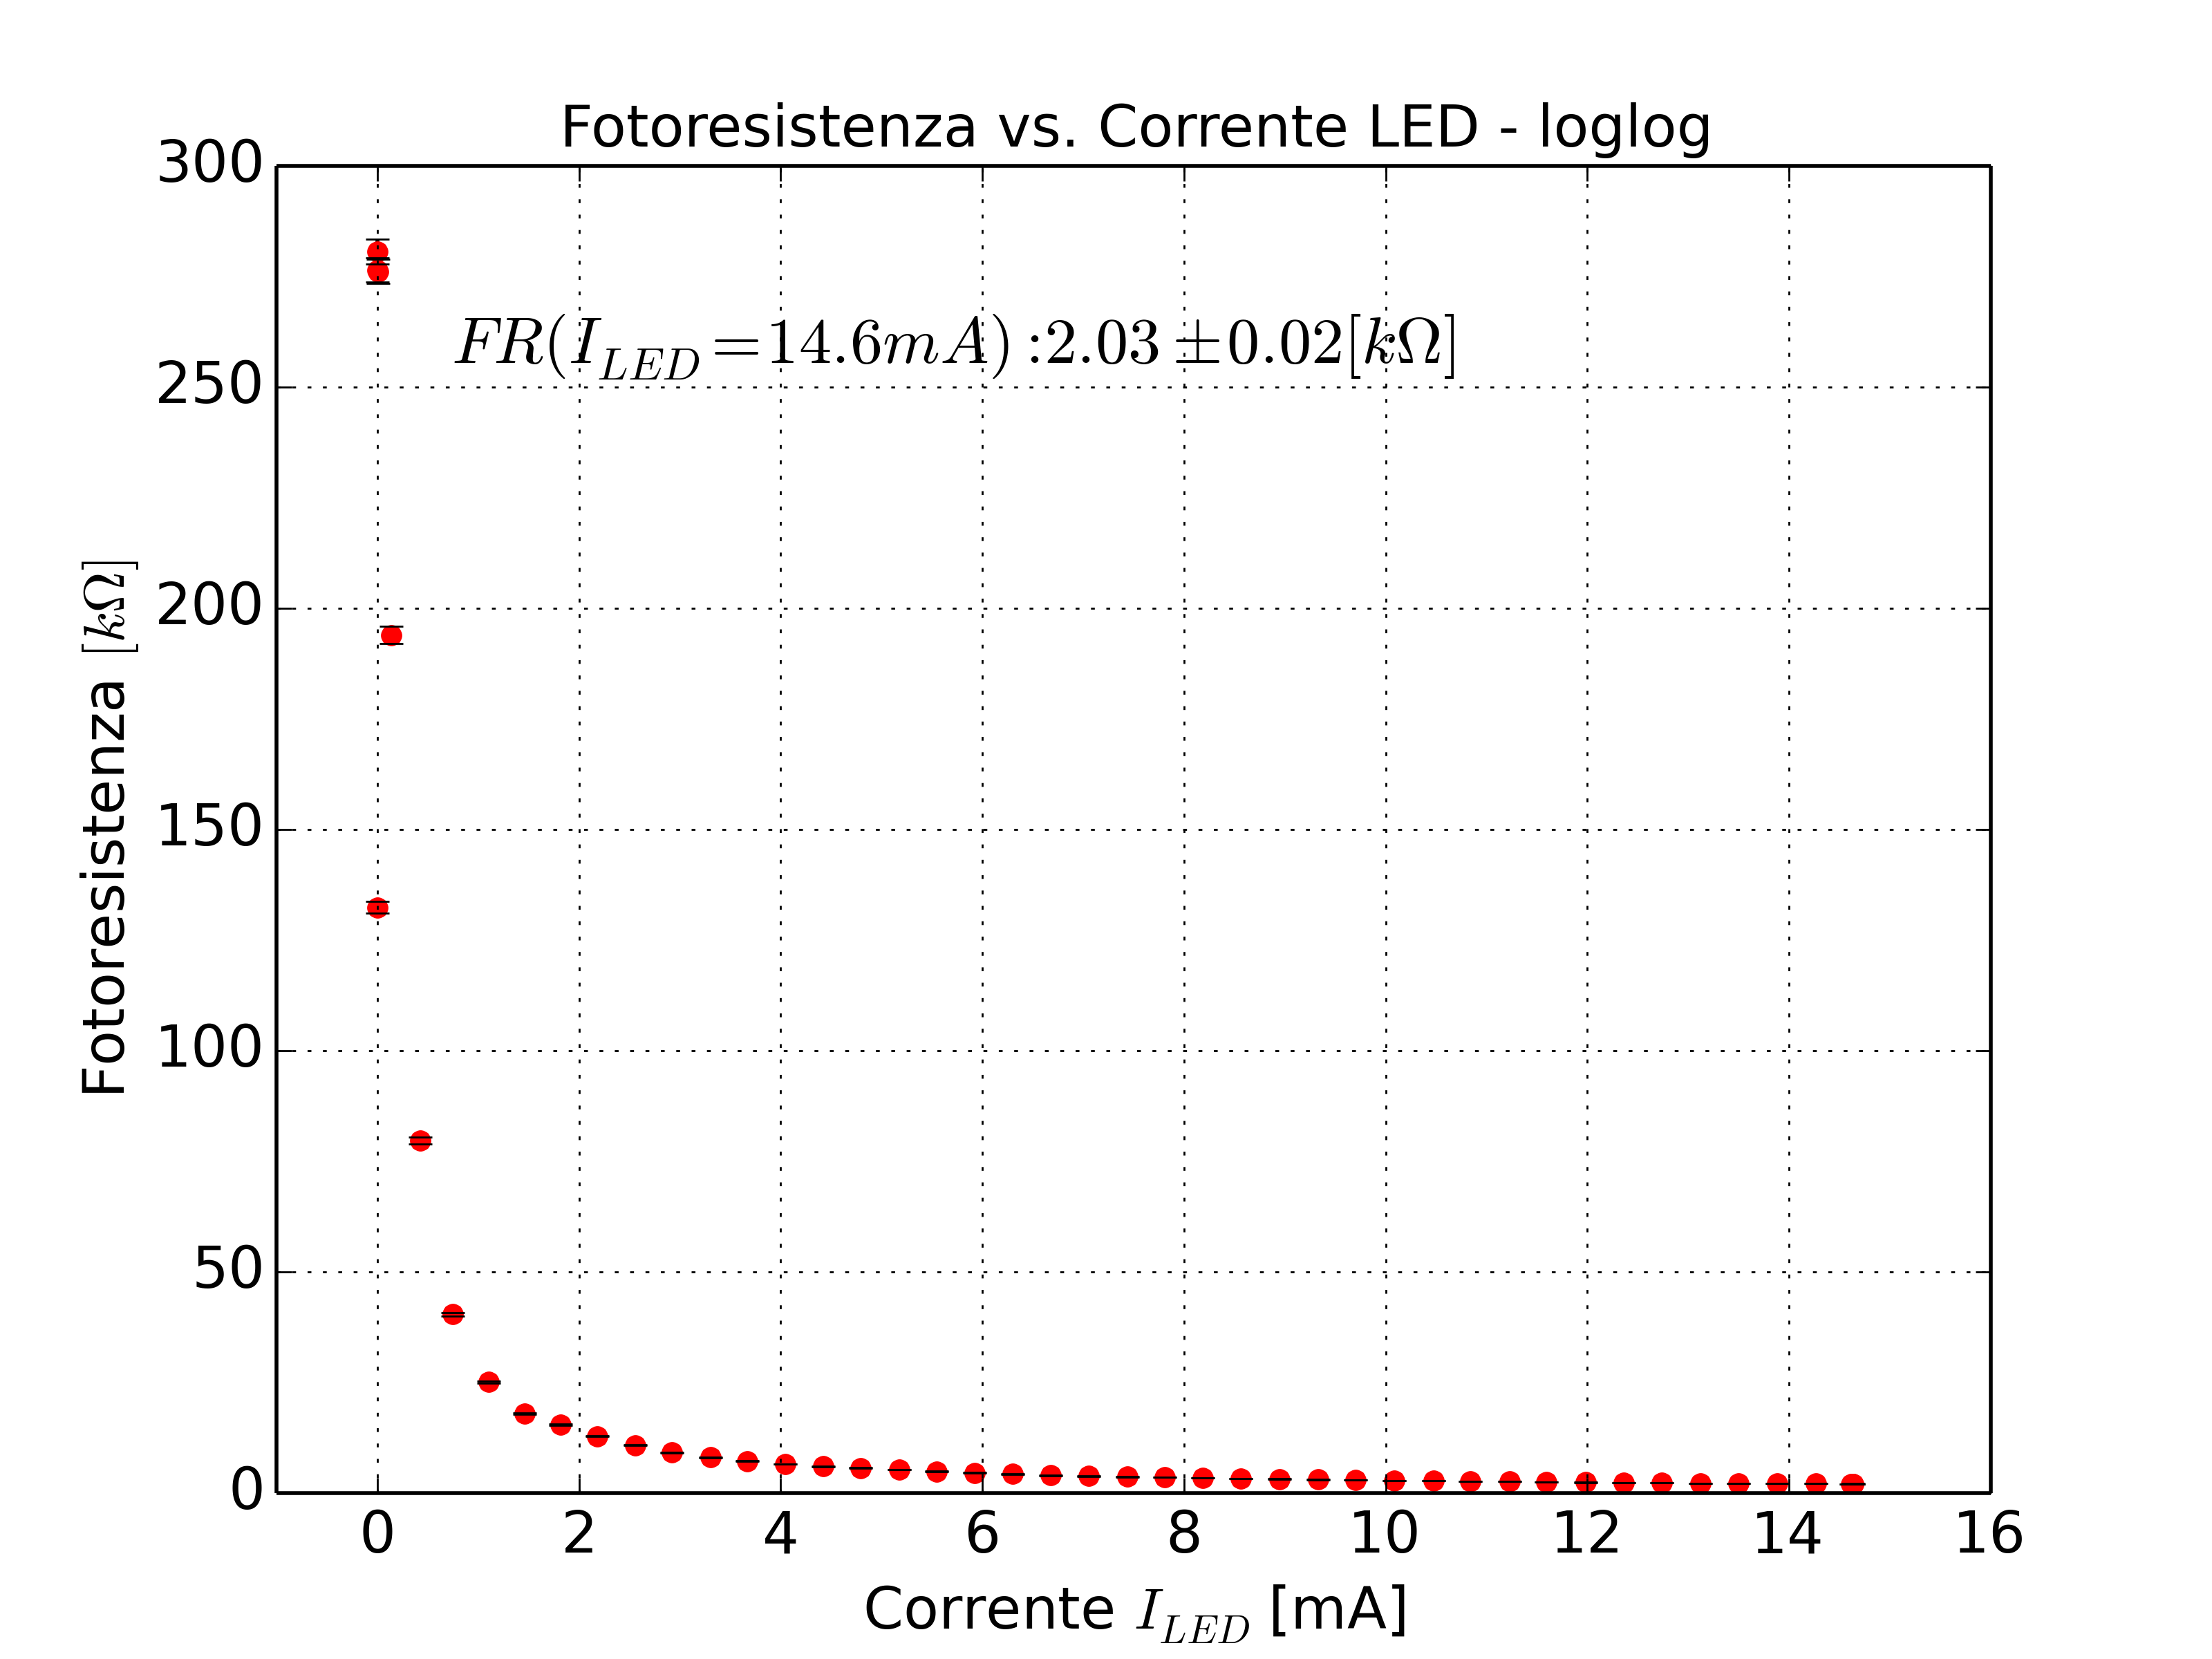
\includegraphics[width=0.9\linewidth]{./plot_FR_vs_ill}
\caption{Fotoresistenza in funzione della corrente nel LED - scala lineare}
\label{fig:plot_FR_vs_ill}
\end{figure}

\begin{figure}
\centering
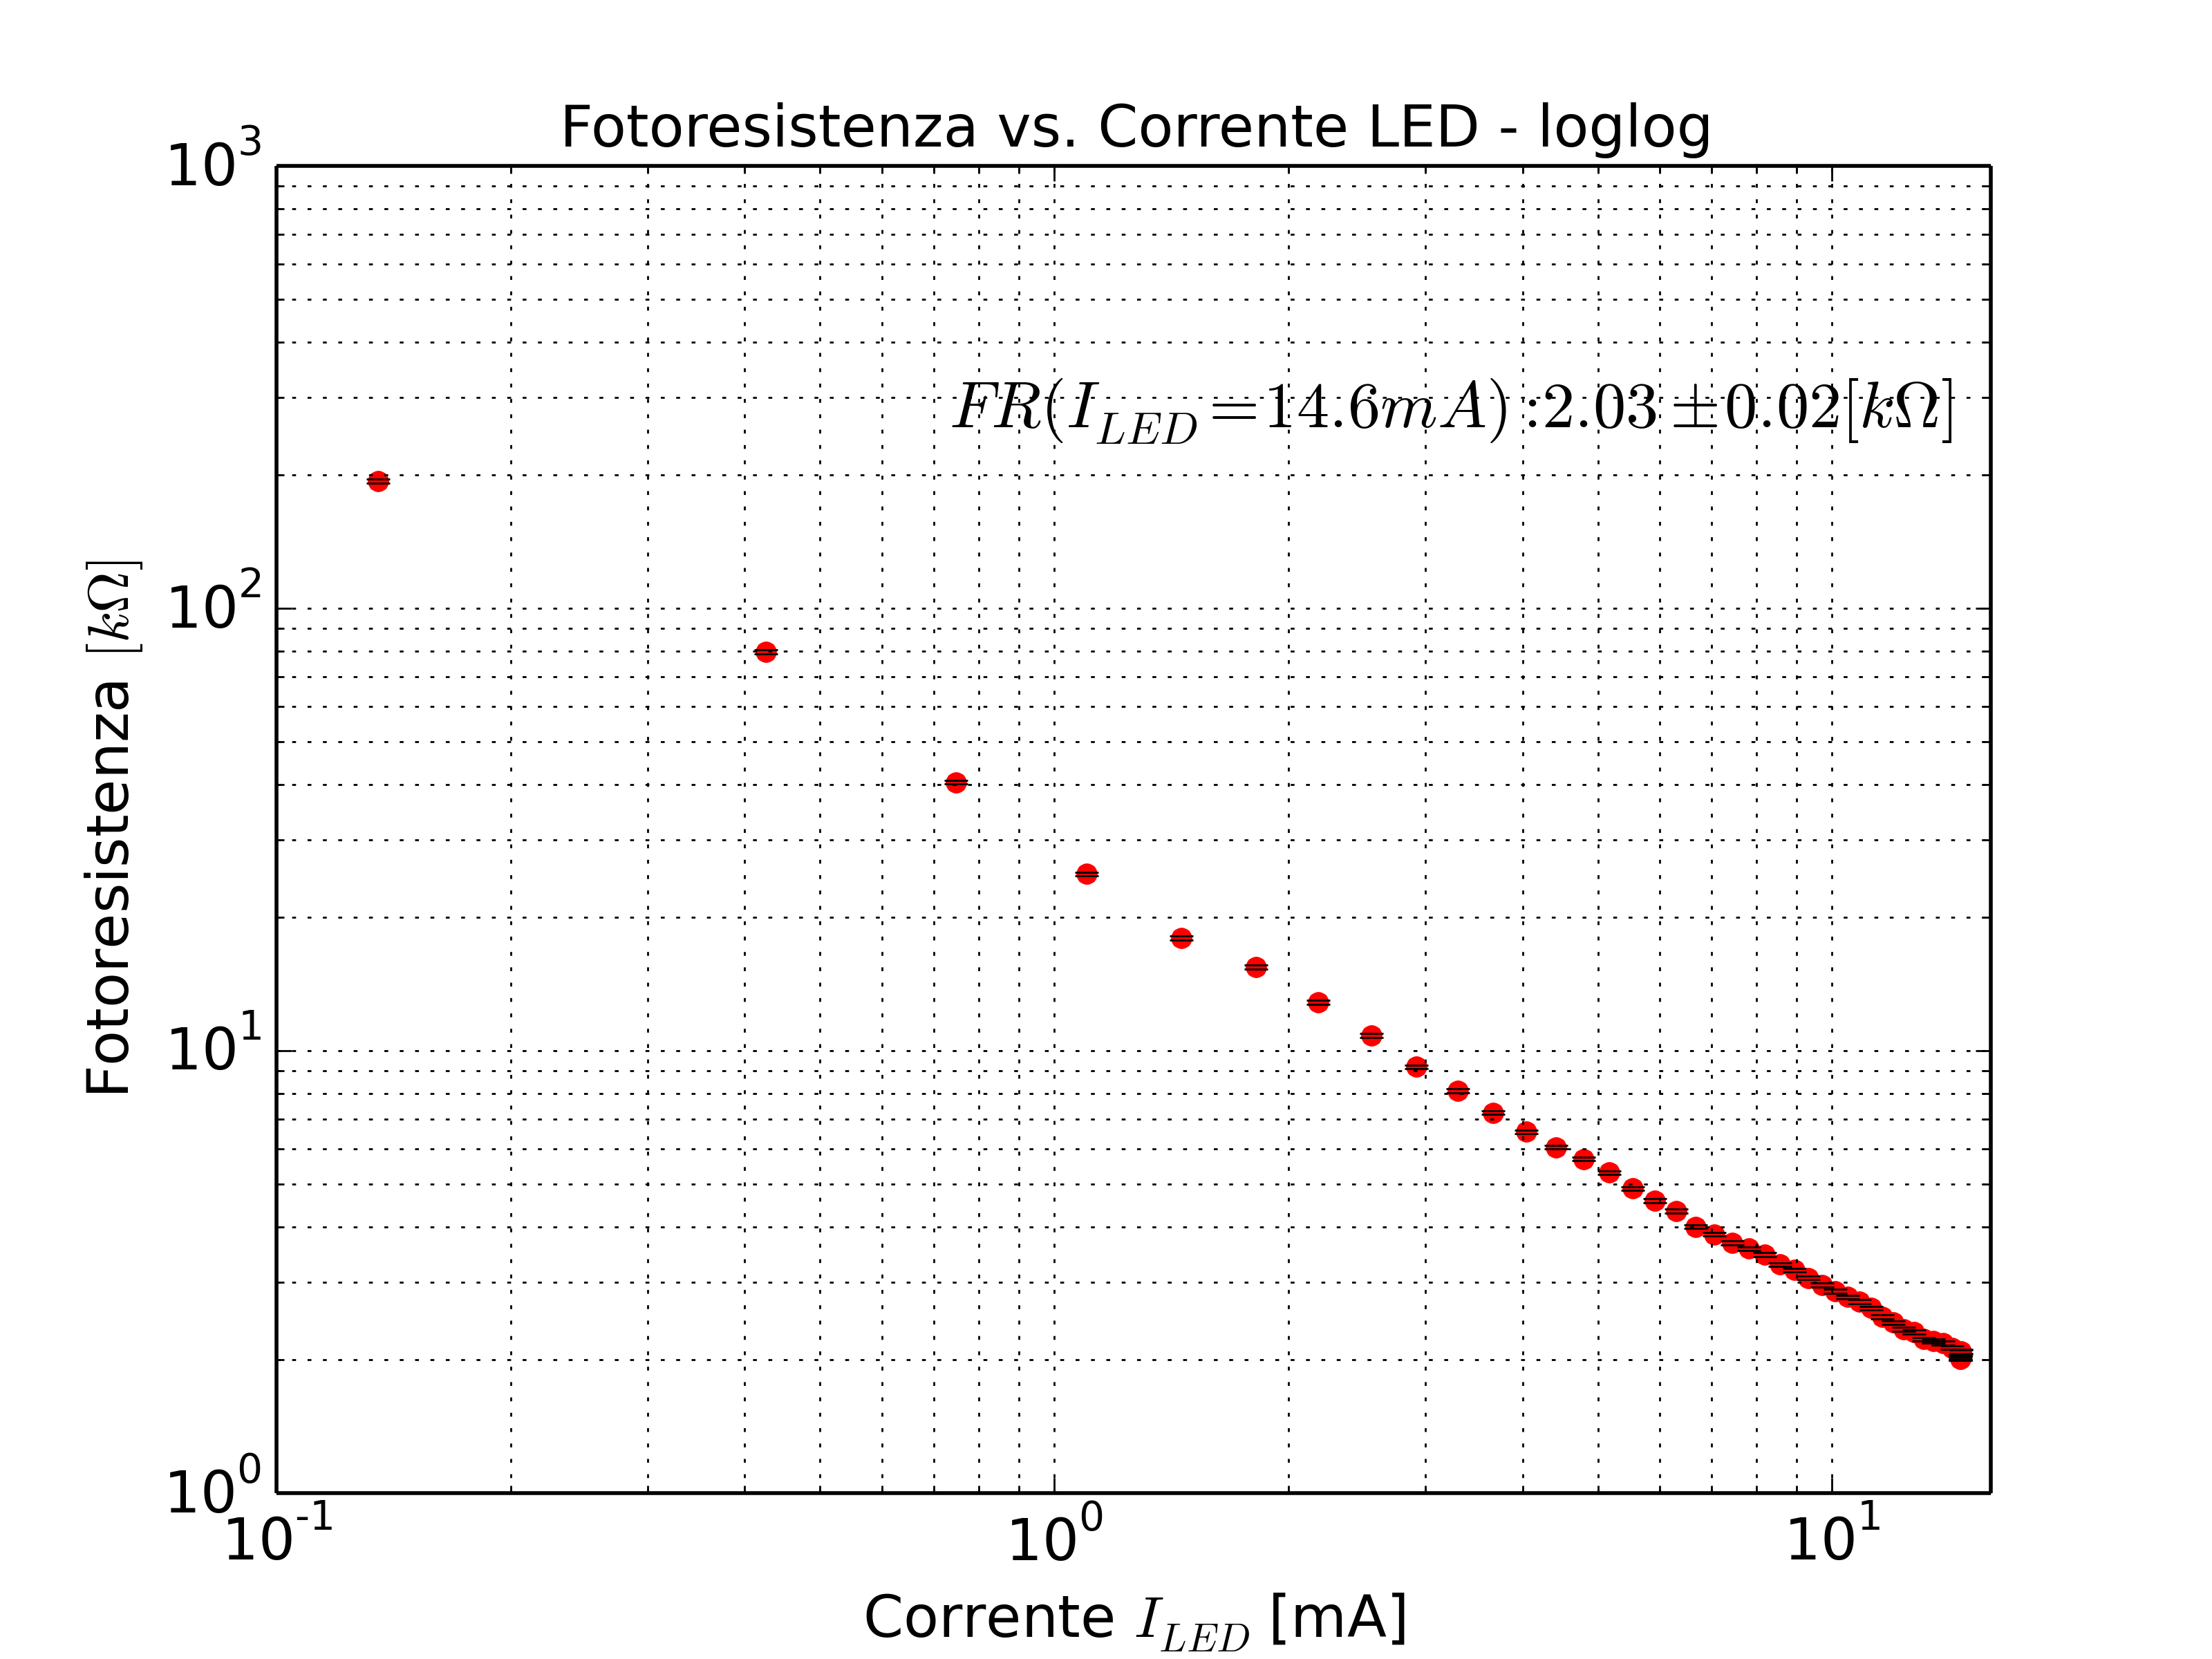
\includegraphics[width=0.9\linewidth]{./plot_FR_vs_ill_loglog}
\caption{Fotoresistenza in funzione della corrente nel LED - scala loglog. Si noti che il coefficiente angolare della retta risulta circa pari a 1, in accordo con quanto aspettato.}
\label{fig:plot_FR_vs_ill_loglog}
\end{figure}

Per verificare queste osservazioni, si è proceduto ad effettuare il fit dei dati sperimentali (escludendo i primi 3 punti poichè non significativi), con una funzione di fit di questo tipo:

\begin{equation}
f(x) = par[0] + \frac{par[2]}{(x + par[3])^{1 + par[1]}}
\end{equation}

dove i parametri 0,3 tengono conto di una traslazione lungo x e lungo y, il parametro 2 di un fattore di forma, il parametro 1 (il più importante) dello scostamento rispetto ad una legge come potenza di x al denominatore. Il risultato del fit (in Figura (\ref{fig:fit_FR_vs_ill})) è abbastanza buono, con una deviazione di 0.27(4) dalla legge aspettata.

\begin{figure}
\centering
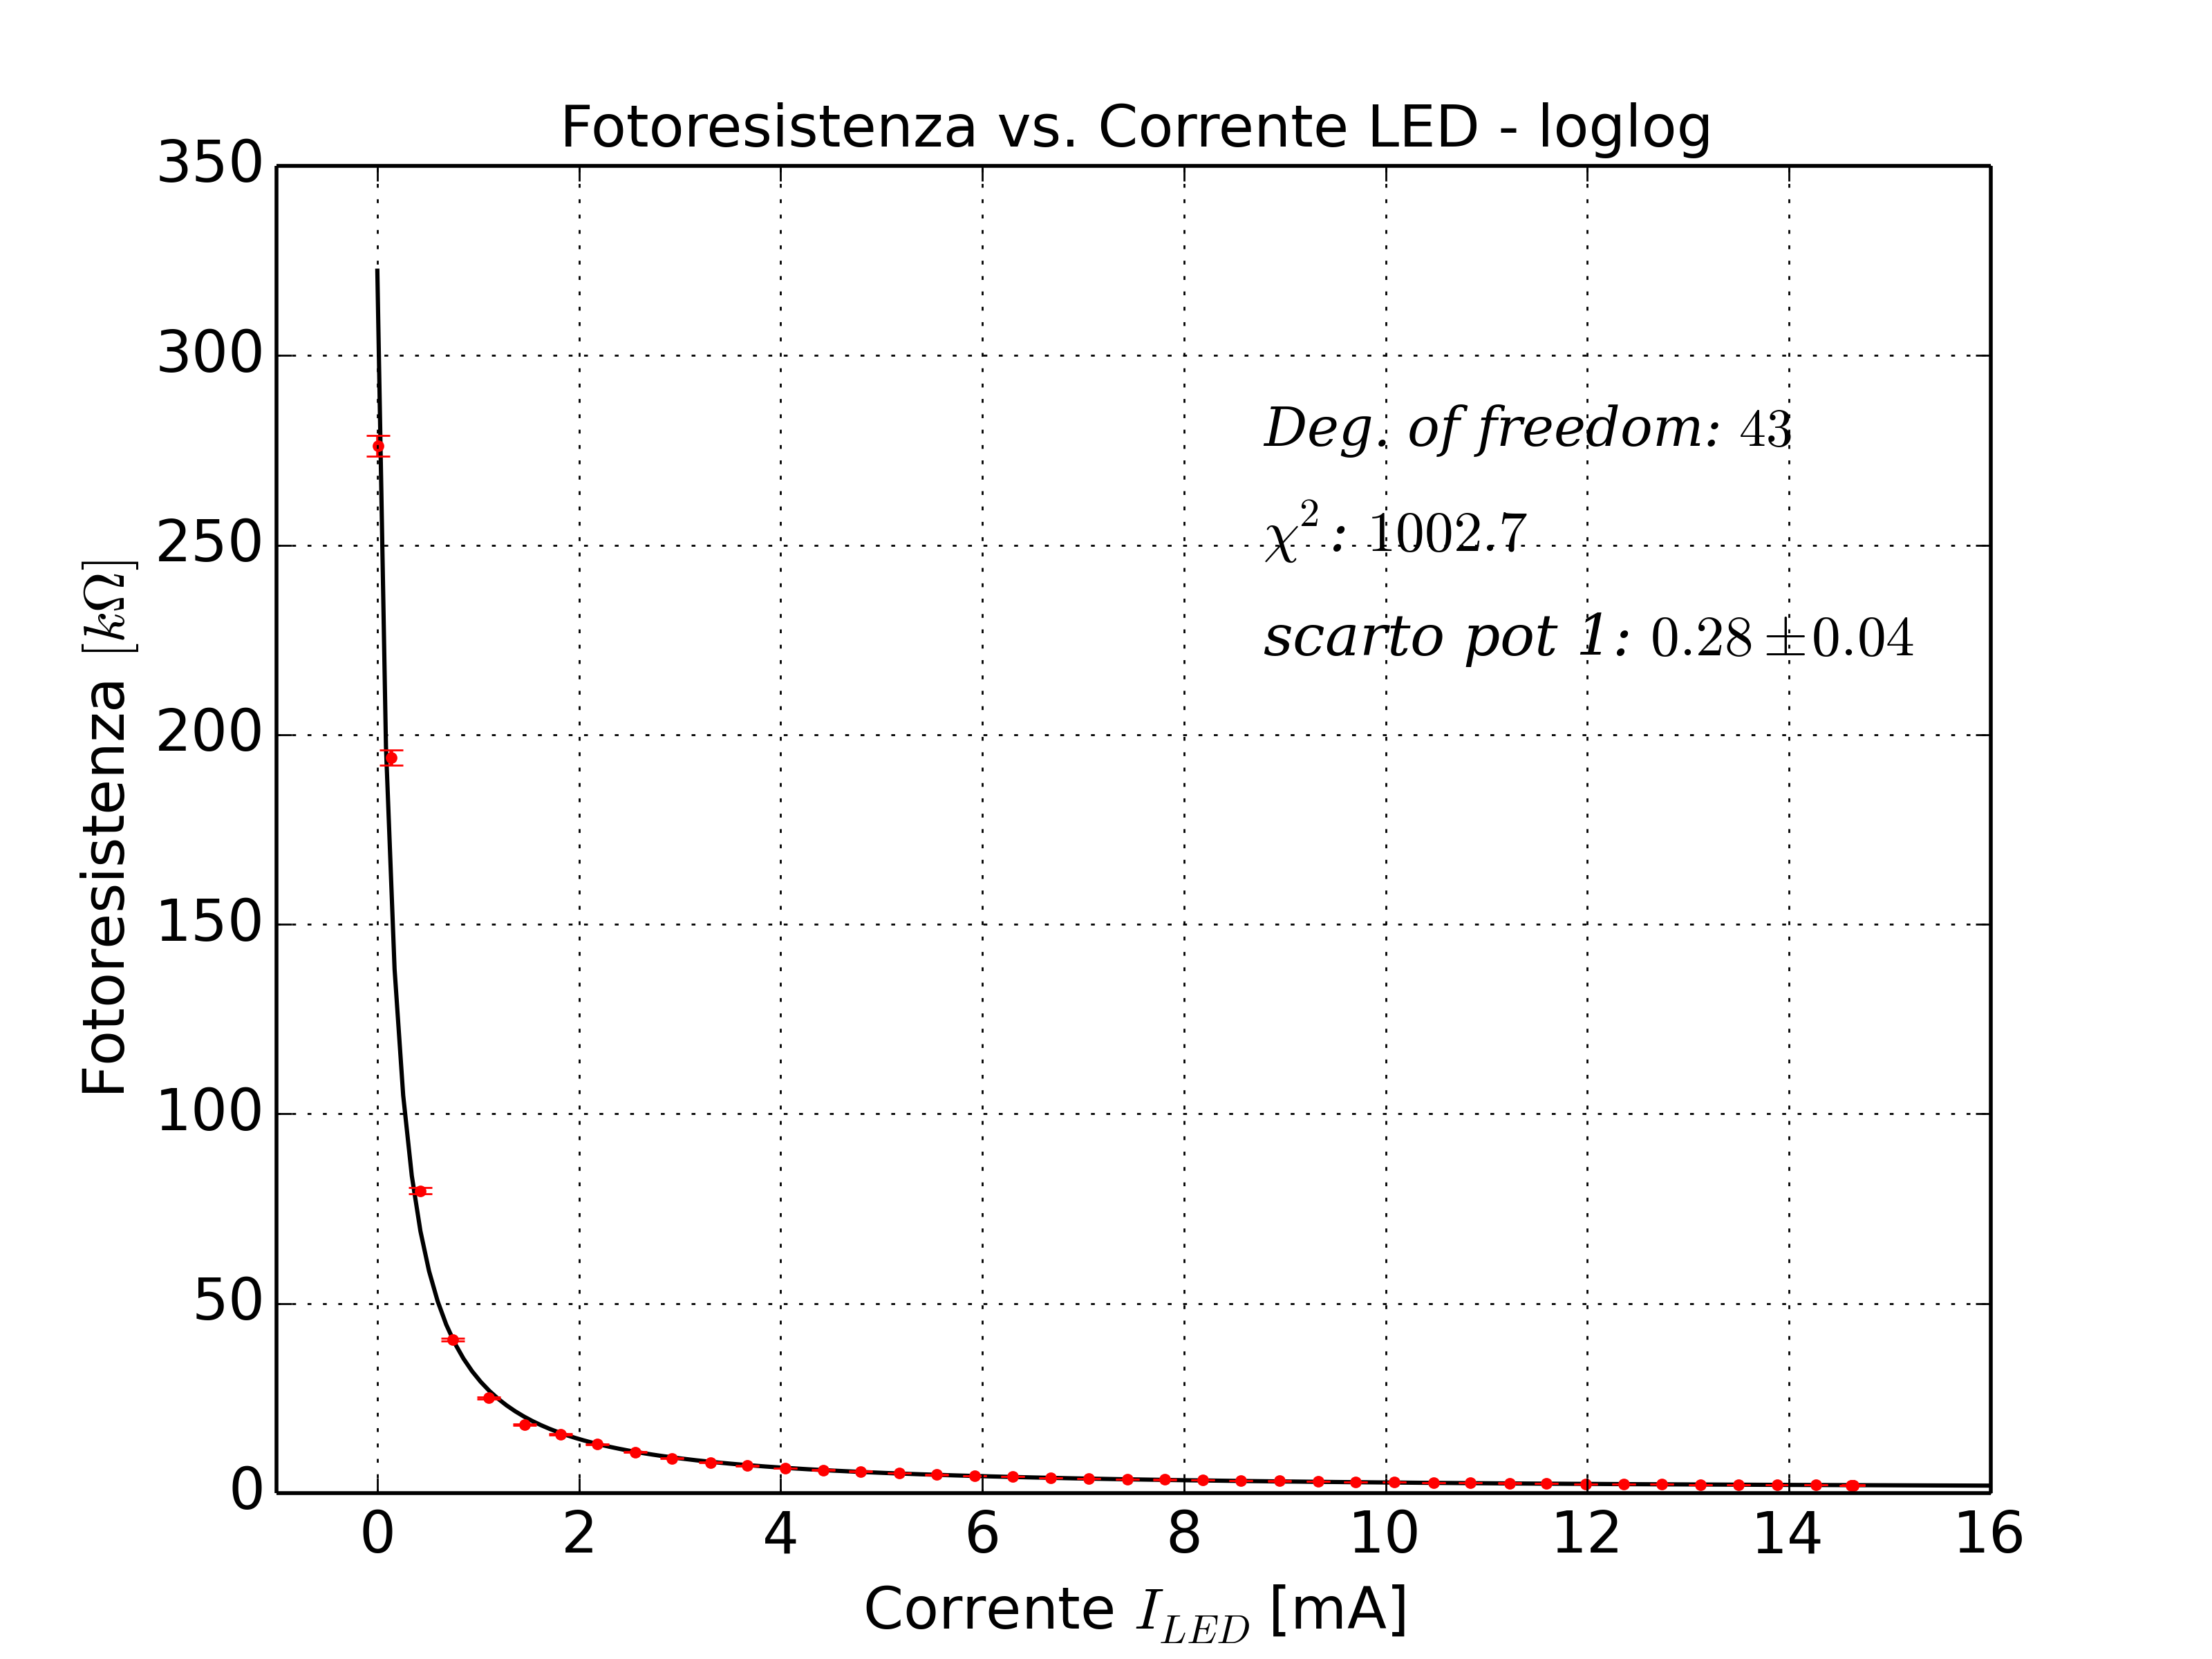
\includegraphics[width=0.9\linewidth]{./fit_FR_vs_ill}
\caption{Fit fotoresistenza in funzione della corrente LED. Deviazione dalla legge 1/x}
\label{fig:fit_FR_vs_ill}
\end{figure}

\section{BONUS: analisi di Fourier del segnale rilevato dalla fotocellula}
In questa sezione, proveremo ad analizzare nel dominio delle frequenze il segnale rilevato dalla fotocellula sotto illuminazione ambientale e flash del cellulare. Si faccia riferimento alla Figura (\ref{fig:illnoncop}) per la tensione rilevata ai capi della fotocella con l'illuminazione delle lampade del laboratorio, e invece alla Figura (\ref{fig:es4_flash_0-005_50k}) per quella del flash. \\

\begin{figure}
\centering
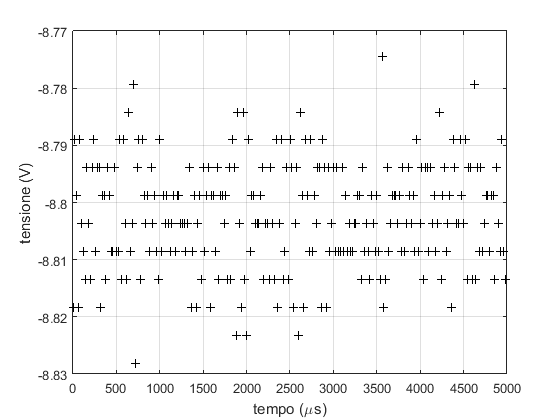
\includegraphics[width=0.8\linewidth]{./es4_flash_0-005_50k}
\caption{Segnale ai capi della fotocellula illuminata dal flash: durata dell'acquisizione 5ms, con sampling rate di 50kS/s}
\label{fig:es4_flash_0-005_50k}
\end{figure}

E' stata fatta l'analisi di Fourier di entrambi i segnali, sfruttando l'algoritmo della \textit{fast fourier transform} (FFT), che utilizza una trasformata discreta. Come ci aspettavamo, nel caso dell'illuminazione del laboratorio, è risultato predominante un segnale a frequenza periodica di 100 Hz, insieme alle armoniche successive (200Hz, 300Hz...) oltre che ad una componente rilevante a frequenza zero, che rappresenta la media del segnale durante tutta l'acquisizione (vedi Figura (\ref{fig:spectral_analysis_flash-senzaflash} )-b). Invece, la FFT del segnale prodotto dal flash della fotocamera ha presentato degli insoliti picchi nelle frequenze comprese fra 6-8kHz: in prima battuta ci saremmo aspettati che il flash venisse alimentato in continua dalla batteria del cellulare (Figura (\ref{fig:spectral_analysis_flash-senzaflash} )-a)). Come ultima annotazione vediamo che quando la cella è illuminata dal flash, non vi sono componenti (evidenti) ascrivibili all'illuminazione delle lampade del laboratorio, che quindi interferiscono molto poco.

\begin{figure}
\centering
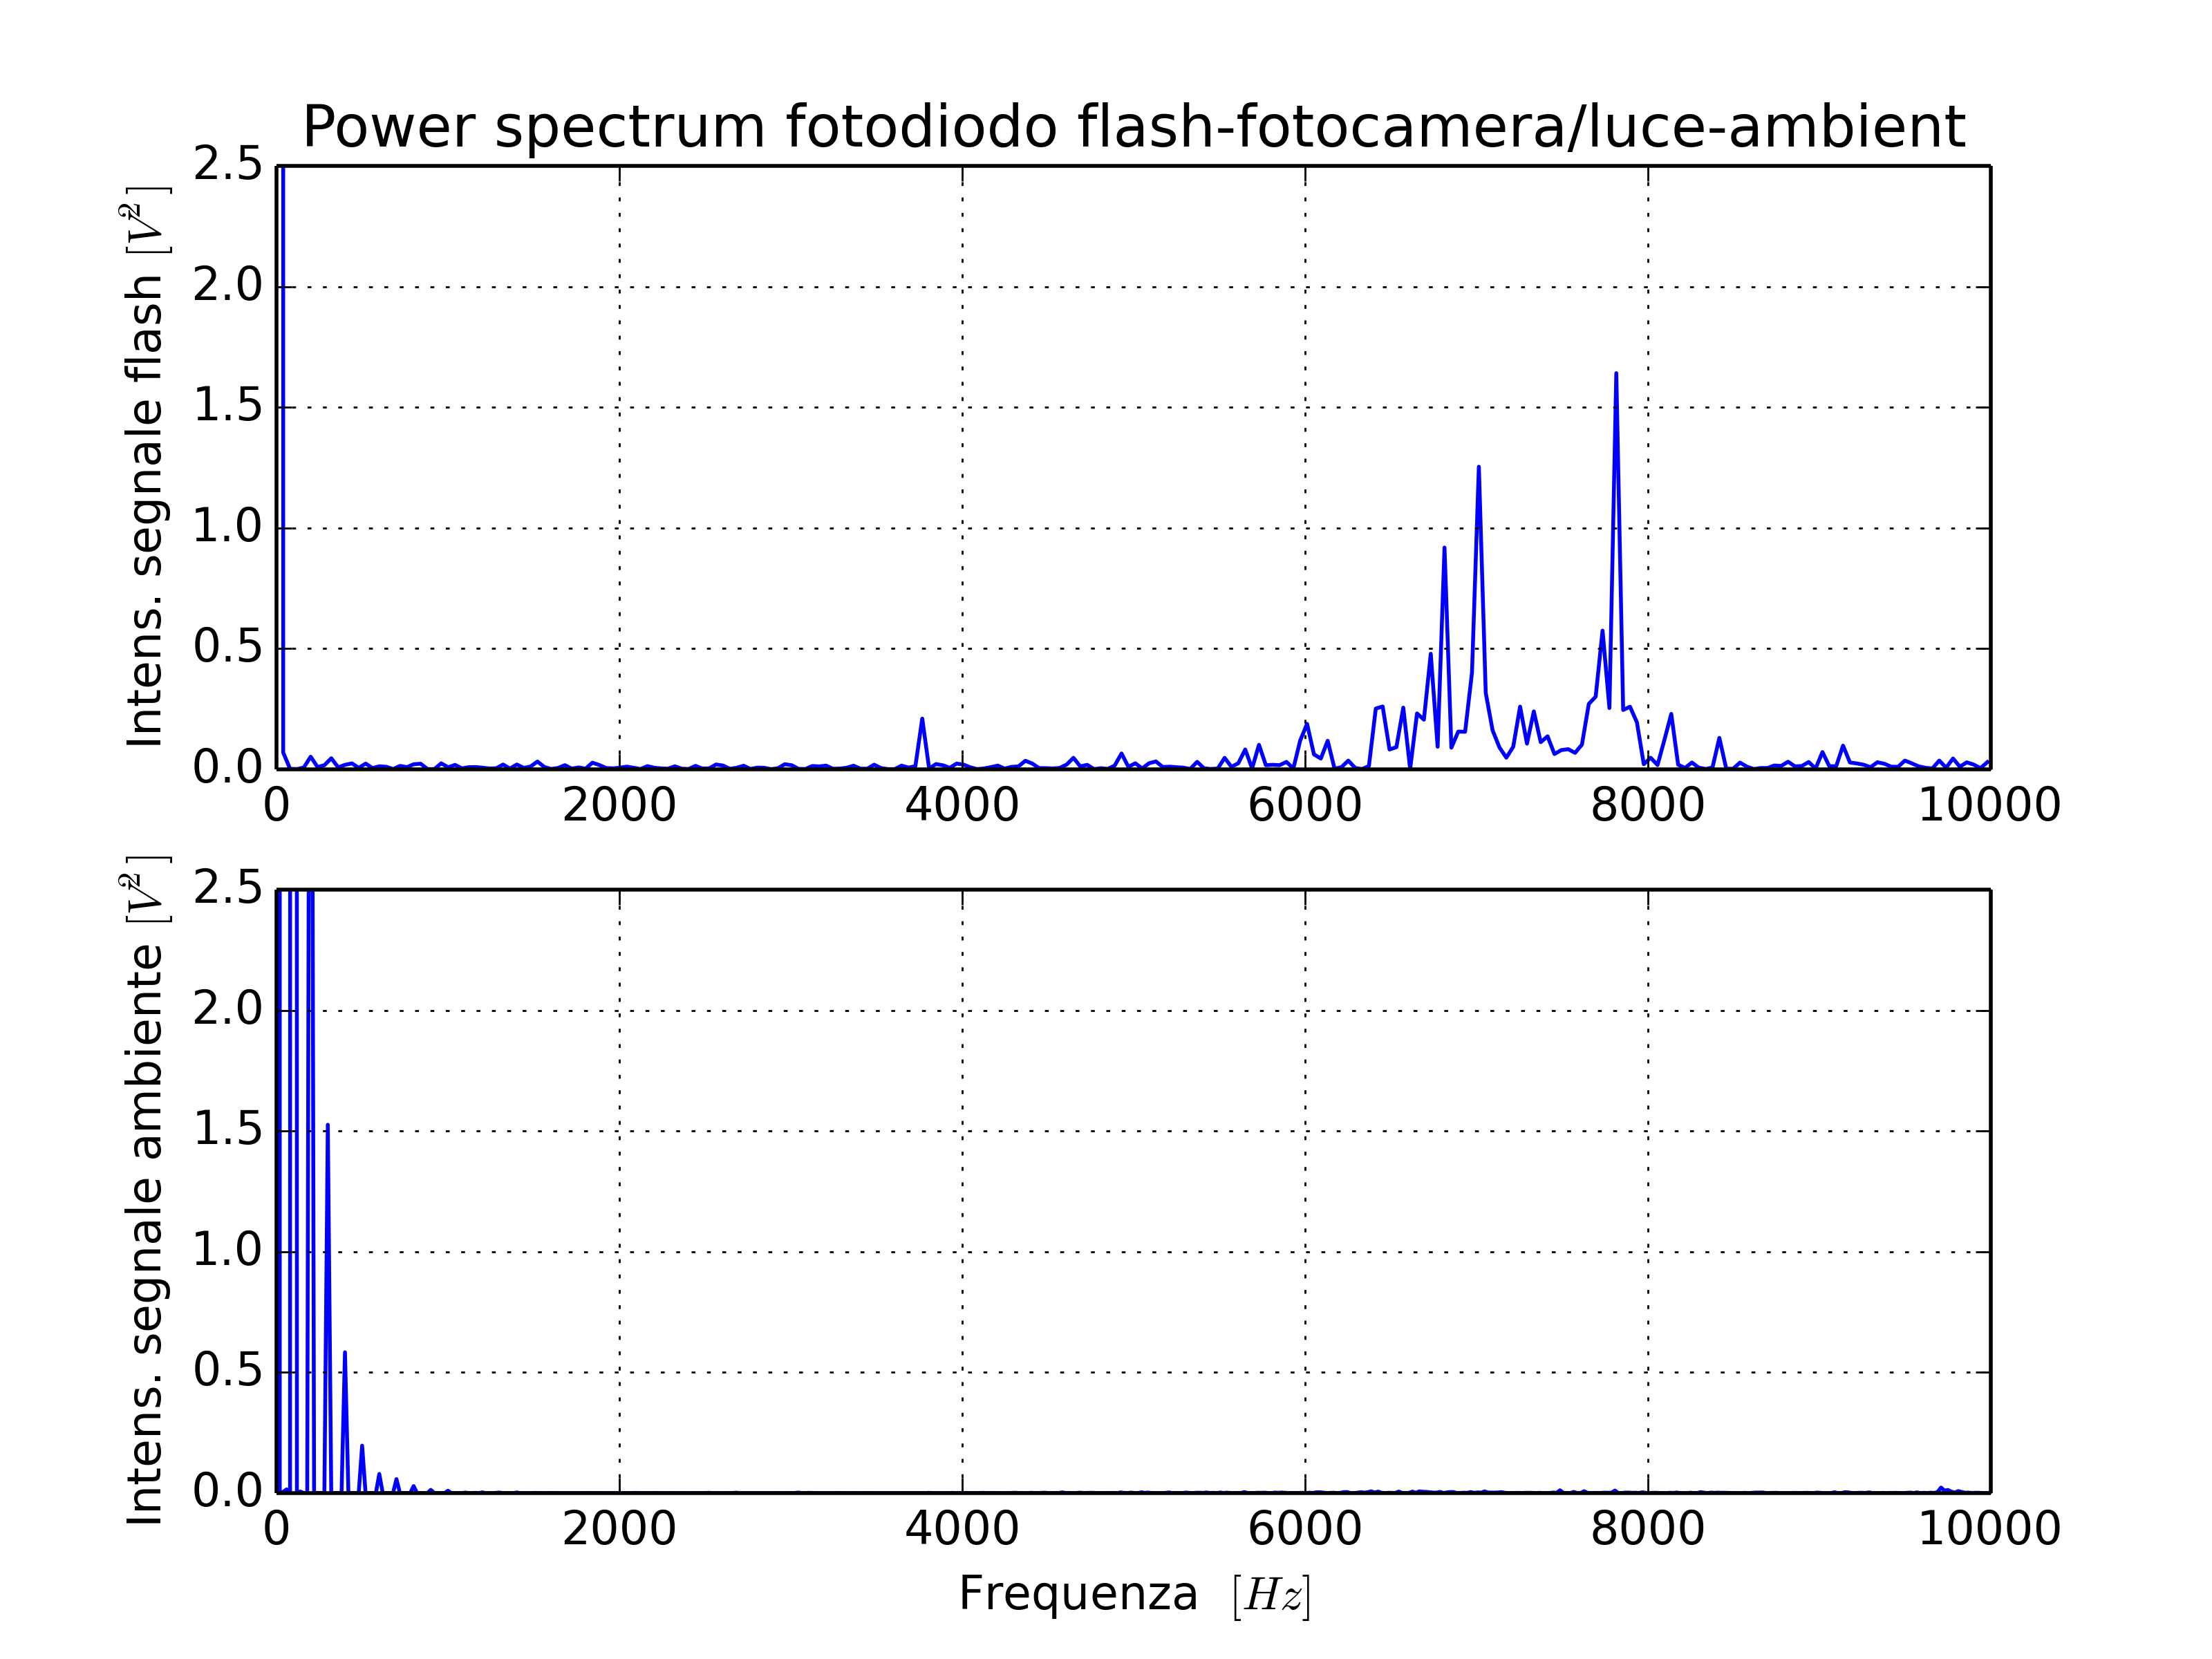
\includegraphics[width=0.8\linewidth]{./spectral_analysis_flash-senzaflash}
\caption{FFT dei segnali prodotti dalla fotocellula sotto luce ambientale e del flash.}
\label{fig:spectral_analysis_flash-senzaflash}
\end{figure}



\begin{thebibliography}{5}

	%Each item starts with a \bibitem{reference} command and the details thereafter.
	\bibitem{HOP96} % Transaction paper
	Datasheet, $\mu $A741 General-Purpose Operational Amplifiers. SLOS094E – NOVEMBER 1970  –REVISED JANUARY 2015.
	\url{http://www.ti.com/lit/ds/symlink/ua741.pdf}

	\bibitem{MJ06} % Conference paper
	Product data sheet: 1N4148 High-speed diodes. NXP Semiconductors 2004 Aug 10.
	\url{http://www.nxp.com/documents/data_sheet/1N4148_1N4448.pdf}

	\bibitem{MJH0} % Conference paper
	Product data sheet: AD711 op-amp.
	\url{http://www.analog.com/media/en/technical-documentation/data-sheets/AD711.pdf}
	
	\bibitem{JH06} % Conference paper
	Product data sheet: OP27 op-amp.
	\url{http://www.analog.com/media/en/technical-documentation/data-sheets/OP27.pdf}
	
	\bibitem{JH6} % Conference paper
	Product data sheet: tl081 op-amp.
	\url{http://www.ti.com/lit/ds/symlink/tl081.pdf}

	\bibitem{M06} % Conference paper
	Paul Horowitz, Winfield Hill - The Art of Electronics. Cambridge University Press (1989).
	
\end{thebibliography}

% Your document ends here!
\end{document}